\documentclass{sig-alternate} 
\usepackage{mathptmx} % This is Times font
\newcommand{\ignore}[1]{}
\usepackage{fancyhdr}
\usepackage[normalem]{ulem}
\usepackage[hyphens]{url}
\setlength{\emergencystretch}{10pt}
\usepackage{graphicx}
\usepackage{multirow}
\usepackage{breakurl}
\usepackage{tabularx}
\usepackage{balance}
\usepackage[nocompress]{cite}
\usepackage{subfig}
\usepackage{hyphenat}
\usepackage{xcolor}
\usepackage{soul}
\usepackage{dcolumn}
\newcolumntype{d}{D{.}{.}{2.1}}
\usepackage{pifont}
\usepackage{flushend}
\usepackage{booktabs}
\usepackage{tikz}
\usepackage{siunitx}
\newcommand*\mycirc[1]{{\large \ding{\numexpr201+#1\relax}}}
% Always include hyperref last
% \usepackage[bookmarks=true,breaklinks=true,letterpaper=true,colorlinks,linkcolor=black,citecolor=blue,urlcolor=black]{hyperref}
% required to break long URLS sanely
% \PassOptionsToPackage{hyphens}{url} \usepackage{hyperref}
\expandafter\def\expandafter\UrlBreaks\expandafter{\UrlBreaks% save the current one 
\do\a\do\b\do\c\do\d\do\e\do\f\do\g\do\h\do\i\do\j% 
\do\k\do\l\do\m\do\n\do\o\do\p\do\q\do\r\do\s\do\t% 
\do\u\do\v\do\w\do\x\do\y\do\z\do\A\do\B\do\C\do\D% 
\do\E\do\F\do\G\do\H\do\I\do\J\do\K\do\L\do\M\do\N% 
\do\O\do\P\do\Q\do\R\do\S\do\T\do\U\do\V\do\W\do\X% 
\do\Y\do\Z\do\*\do\-\do\~\do\'\do\"\do\-}%

% Ensure letter paper
\pdfpagewidth=8.5in
\pdfpageheight=11in
\pagenumbering{arabic}

%%%%%%%%%%%---SETME-----%%%%%%%%%%%%%
\newcommand{\microsubmissionnumber}{265}
%%%%%%%%%%%%%%%%%%%%%%%%%%%%%%%%%%%%

\newcommand*\circled[1]{\tikz[baseline=(char.base)]{
  \node[shape=circle,draw,inner sep=1pt] (char) {#1};}}

\fancypagestyle{firstpage}{
  \fancyhf{}
  \renewcommand{\headrulewidth}{0pt}
  \fancyhead[C]{\vspace{15pt}\normalsize{Accepted for Publication at MICRO 2017 -- Non-Final Draft -- Do Not Distribute!!}} 
  \fancyfoot[C]{\thepage}
}

%\title{NUMA-Aware GPUs for Multi-Socket Designs}
\title{Beyond the Socket: NUMA-Aware GPUs}
\vspace{-.5in}

\author{
Ugljesa Milic$^{\dagger\ddagger}$,
Oreste Villa$^{\dagger}$,
Evgeny Bolotin$^{\dagger}$,
Akhil Arunkumar$^{\dagger\star}$,\\\\
Eiman Ebrahimi$^{\dagger}$,
Aamer Jaleel$^{\dagger}$,
Alex Ramirez$^{\dagger\ast}$,
David Nellans$^{\dagger}$
\\\\
$^{\dagger}$NVIDIA, $^{\ddagger}$Barcelona Supercomputing Center, $^{\star}$Arizona State University, and $^{\ast}$Google\\
% \{ovilla,ebolotin,eebrahimi,ajaleel,dnellans}\\@nvidia.com,ugljesa.milic\\@bsc.es,alex.ramirez\@google.com
}

\begin{document}
% \thanks{This research was supported in part by the United States Department of Energy. The views and conclusions contained in this document are those of the authors and 
% should not be interpreted as representing the official policies, either expressed or implied, of the U.S. Government.}
\maketitle
\thispagestyle{firstpage}
\pagestyle{plain}
\begin{abstract}
GPUs achieve high throughput and power efficiency by employing many small single 
instruction multiple thread (SIMT) cores.  To minimize scheduling logic and 
performance variance they leverage strong data parallelism exposed via the 
programming model attached to a uniform memory access system (UMA) With Moore's 
law slowing, for GPUs to continue scaling performance (which largely depends on 
SIMT core count) they are likely embrace multi-socket designs where more 
transistors are more readily available. However when moving to multi-socket 
designs, maintaining the illusion of a uniform memory system becomes 
increasingly difficult.  In this work we investigate future multi-socket NUMA 
GPU designs and show that significant changes are needed to the GPU interconnect 
and caching systems to achieve performance scalability. We show that application 
phase effects can be exploited, allowing GPU sockets to dynamically optimize 
their individual interconnect and cache policies to minimize the impact of 
non-uniform memory access (NUMA) effects. Our NUMA-aware GPU is able to 
outperform current UMA based designs by XXX\%, XXX\%, and XXX\% and achieves 
XXX\%, XXX\%, and XXX\% of theoretical application scalability in 2, 4, and 8 
socket designs respectively.  Implementable today, NUMA-aware multi-socket GPUs 
may be a promising candidate for scaling GPU performance beyond a single die.
\end{abstract}
\section{Introduction}
\label{introduction}

In the last 10 years GPUs computing has transformed the high performance 
computing, machine learning, and data analytics fields that were previously 
dominated by CPU-based 
installations~\cite{intersect360,cudnn,Lavin15b,SimonyanZ14a}. Many systems now 
rely on a combination of GPUs and CPUs to leverage high throughput data parallel 
GPUs with latency critical execution occurring on the CPUs. In part, 
GPU-accelerated computing has been successful in these domains because of native 
support for data parallel programming languages~\cite{CUDA7,OPENCL} that reduce 
programmer burden when trying to scale programs across ever growing data sets.

\begin{figure}[t]
\centering
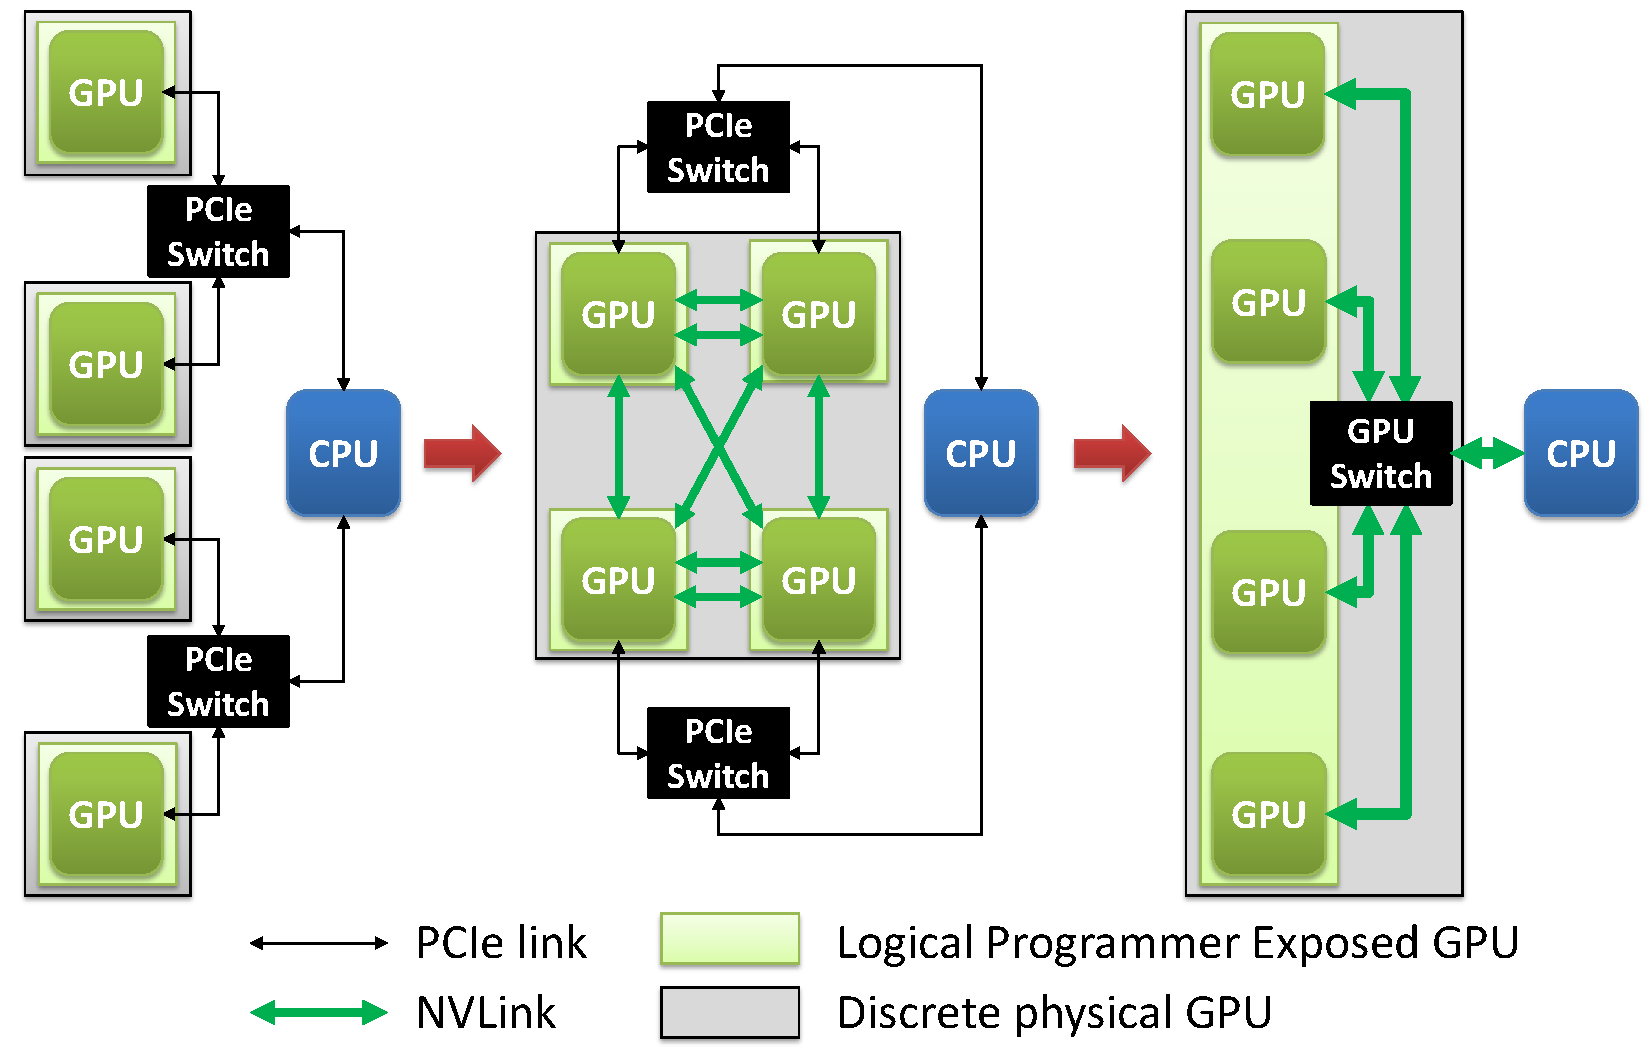
\includegraphics[width=1.0\columnwidth]{figures/inter_gpu_connections.pdf}
\caption{The evolution of GPUs from multiple discrete PCIe devices to 
single logical, multi-socket accelerators utilizing switched interconnects.}
\label{fig:systemdiagram}
\vspace{-.2in}
\end{figure}

Nevertheless, with GPUs nearing the reticle limitation for maximum die size and 
the transistor density growth rate slowing down~\cite{mooredead2016}, developers 
looking to scale the performance of their single GPU programs are in a 
precarious position. Multi-GPU programming models support explicit programming 
of two or more GPUs, but it is challenging to leveraging mechanisms such as 
Peer-2-Peer access~\cite{NVIDIAP2P} or a combination of MPI and 
CUDA~\cite{NVIDIAMPI} to manage multiple GPUs. These programming extensions 
enable programmers to employ more than one GPU for high throughput computation, 
but they require re-writing of traditional single GPU applications which has 
slowed their adoption rate.

Recently GPUs have started to transition from using the PCIe peripheral 
interface to having single protocol interconnections between both the GPUs and 
CPUs~\cite{dgx,SierraHPC,AMDINFINITYFABRIC}, as shown in 
Figure~\ref{fig:systemdiagram}. As a result, the physical interface of GPUs is 
transitioning away from a discrete pluggable PCIe card into a high pin-count 
socketed module. This socketed interface is required 
not only for power delivery but because
printed circuit board (PCB) level integration is needed to provide
interconnect bandwidth that is up to an order of magnitude higher than PCIe
connections. The evolution of GPUs from single pluggable devices to closely
coupled multi-socket designs is a natural progression as GPU--GPU and CPU--GPU
link bandwidth becomes a performance critical system component.

The onset of multi-socket GPUs provides a pivot point for GPU and system 
vendors. On one hand, vendors can continue to expose multi-socket GPUs as 
individual GPUs and force developers to use multiple programming paradigms to 
leverage multiple GPUs. On the other, vendors could expose multi-socket 
designs as a single non-uniform memory access (NUMA) GPU resource.  By 
extending the single GPU programming model to multi-socket GPUs,  applications 
can scale beyond the bounds of Moore's law, while simultaneously retaining the 
programming interface that GPU developers have become accustomed.

Several groups have previously examined aggregating multiple GPUs together under 
a single programming model~\cite{lee2013transparent,Cabezas2015}; however this 
work was done in an era where GPUs had limited memory addressability and relied 
on high latency, low bandwidth PCIe interconnects. As a result, prior work 
focused primarily on improving the multi-GPU programming experience rather than 
achieving highly scalable performance. Building upon this work, we propose a 
multi-socket \textit{NUMA-aware} GPU architecture and runtime that aggregates 
multiple GPUs into a single programmer transparent logical GPU. We show that in 
the the era of unified virtual addressing~\cite{UVM}, cache line addressable 
high bandwidth interconnects~\cite{NVLINK}, and dedicated GPU and CPU socket PCB 
designs~\cite{SierraHPC}, scalable multi-GPU performance may be achievable under 
existing single GPU programming models. In this work, we make the following 
contributions:

\begin{itemize}

\item We show that traditional software NUMA memory placement and 
scheduling policies are not sufficient for multi-socket GPUs to achieve 
performance scalability.  We then demonstrate that intersocket bandwidth will be 
the primary performance limiter in future NUMA GPUs.

\item By exploiting program phase behavior we show that intersocket links (and 
thus BW) should be dynamically varied at runtime to maximize link 
utilization. Moreover, we show that link policy must be determined on a per 
GPU basis, as global policies fail to capture per GPU phase behavior.

\item We show that both the GPU L1 and L2 caches should be made NUMA-aware 
and dynamically adapt their caching policy to minimize NUMA effects. We demonstrate
that in NUMA GPUs, extending existing GPU cache coherence protocols
across multiple sockets scales is a good design choice, despite the overheads.

\item We show that multi-socket NUMA-aware GPUs can allow traditional 
GPU programs to scale efficiently to as many as 8 GPU sockets, providing significant 
headroom before developers must re-architect applications to obtain additional performance.

\end{itemize}

\section{Motivation and Background}
\label{background}

Single GPU performance has been scaling very well amassing a significant
growth in per-GPU transistor count and DRAM BW. For example a 2010 Nvidia's
529mm\textsuperscript{2} Fermi GPUs integrated 1.95B transistors with 180 GB/s
DRAM bandwidth, while 2016 Nvidia 610 mm\textsuperscript{2} Pascal GPUs reached
a 12B transistor count with 720 GB/s memory bandwidth. Unfortunately transistor density
growth slows down and expected to come to a halt at 7nm. Moreover, as GPU die sizes
have been also increasing over the past generations, this growth is expected to
slow down due to limitations in lithography and manufacturing costs. 
Without larger or denser dies, GPU manufacturers are likely to turn to 
alternative technologies such as the tried and trued solution from CPU world,
the \textit{multi-socket GPUs}, to keep scaling effective GPU perfromance via 
growing overall transistor counts and DRAM bandwidths. 

%One moving to 3D die-stacking as a solution for continued transistor growth. 
%Unfortunately 3D die-stacking still has a significant number of engineering 
%challenges related to power delivery, energy density, and 
%cooling~\cite{verbree2010cost} when employed in maximal die-sized chips such as 
%GPUs and moving beyond a 2 high stack to 4 or 8 stacks will be even more 
%difficult. Because of these challenges, 
%GPU manufacturers are likely to 
%consider a tried and trued solution in the CPU world to gain additional 
%transistor count, \textit{multi-socket GPUs}.

\begin{figure}[t] 
    \centering
    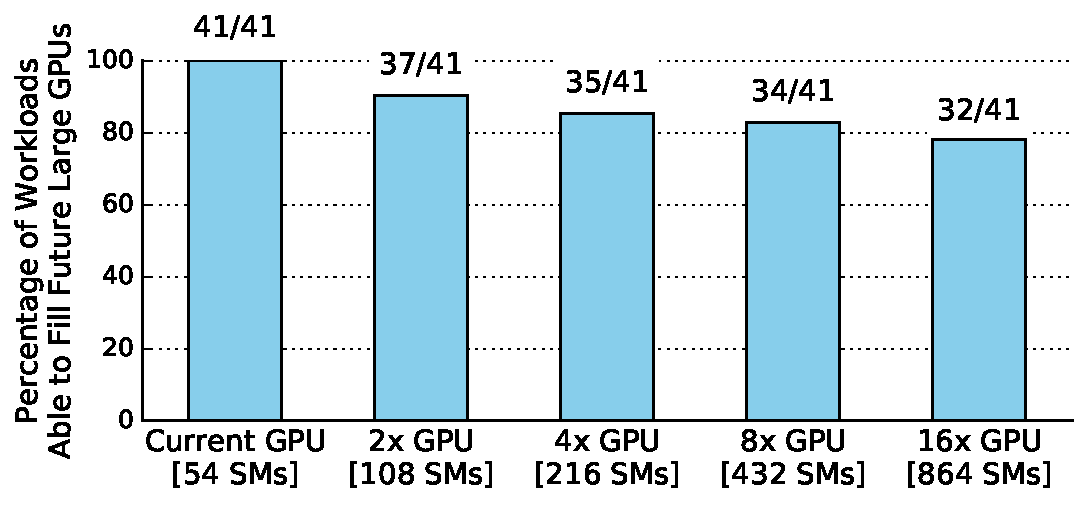
\includegraphics[width=1.0\columnwidth]{figures/plot_ctas_per_sm.pdf}
    \caption{Do we have enough CTAs to fill bigger GPUs.}
    \label{fig:ctas}
\end{figure}

\begin{figure*}[tp] 
    \centering
    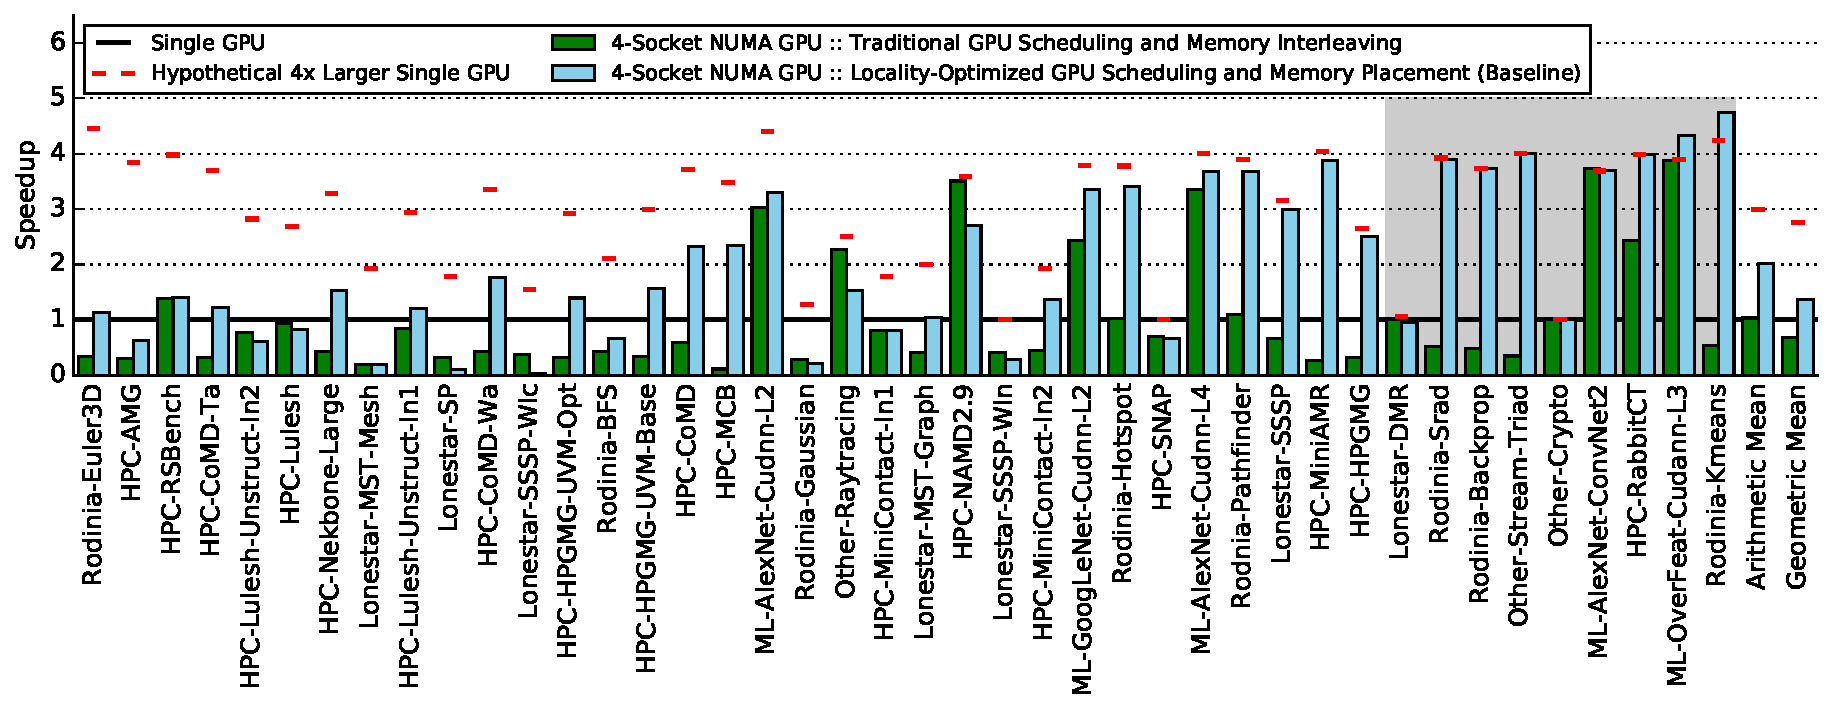
\includegraphics[width=1.0\linewidth]{figures/plot_different_baselines.pdf}
    \caption{Relative performance of a 4-socket NUMA GPU using to a single GPU 
and a hypothetical 4$\times$ larger (all resources scaled) single GPU showing 
upper bound of performance this application can achieve via GPU hardware 
scaling. For the Locality-Optimized design, applications shown in grey 
achieve already 99\% of theoretical scaling (\emph{red dash}) without 
microarchitectural modification.}
    \label{fig:motivation}
\end{figure*}

The evolution of GPU computing has moved from it being a PCIe attached peripherals 
to computing platforms designed around the GPU as the primary computing engine. 
Such systems epmloy custom PCB designs that accommodate multiple high pin count socketed 
GPUs~\cite{DGX} with inter-GPU interconnects resembling QPI or 
Hypertransport~\cite{INTELQPI,AMDHT} much more than legacy PCIe interfaces.  
Despite the improvement in hardware capabilities, to-date these multi-GPU 
solutions have been exposed as a collection of single GPU solutions with improved GPU--GPU 
interconnects. While multi-GPU systems can provide high aggregate throughput, 
the programming models for multi-GPU systems has diverged from the single GPU 
programming model and requires layering additional software runtimes like MPI 
or openshmem on top of the native GPU programming interfaces such as CUDA or openCL.
By requiring re-writing of the GPU application to enable multi-GPU performance, 
many applications are never ported to use multiple GPUs.

In this work, we examine the performance achievable by architecting a 
multi-socket NUMA-aware single GPU.  Building upon existing work in the 
NUMA-CPU and GPU community, we first describe the basic multi-socket GPU runtime 
that allows a multi-socket GPU system to be exposed to GPU developers as a 
single GPU and exploits some well known scheduling and memory locality 
optimizations for NUMA systems. We then look at the performance implications 
that this multi-socket NUMA design has on applications that have been optimized 
for a traditional single GPU.  We identify that current GPU interconnect 
utilization and cache policies are sub-optimal for a multi-socket NUMA GPU and 
show how these problems can largely be overcome with architectural innovation.  
Finally, we examine the scaling efficiency of a multi-socket NUMA-aware GPU to 
understand if NUMA-aware GPUs will see significantly improve performance  
without any code-rewriting required by the application programmer.


----------Evgeny ---- 
the following paragraphs moved from next section, need to be merged here or in
Intro ----------

To improve the performance of our
basic TMS-GPU implementation we propose two classes of improvements that 
leverage application phasing to reduced the effective NUMA penalty.  First, in 
Section~\ref{interconnect} we examine the ability of a switch connected GPU to 
dynamically change its interconnect signaling from a balanced up and down 
stream bandwidth design, to allowing flexible re-partitioning of these channels.  
When bi-directional bandwidth is observed to be under-utilized, the direction 
which has excess capacity can be re-assigned to support the oversubscribed 
channels. This allows any individual GPU to improve its bandwidth utilization at 
times when it finds itself most bandwidth constrained.

Second, because we observe that inter-GPU bandwidth has a strong correlation to
overall multi-socket GPU performance we investigate the performance impact of
enabling multi-socket GPU cache coherence in Section~\ref{caching}.  We propose
extending the software based L1 coherence into the L2 caches of multi-socket
GPUs.  By extending this coherence, the L2 caches of each GPU socket move from
being memory-side, where coherence is not needed, to GPU-side, where coherence
guarantees are required in the same manner as current GPU L1 caches.  We
evaluate the effect of this coherence overhead on multi-socket GPUs and show
that because of the GPU's weak coherence guarantees multi-socket coherence on
GPUs should scale significantly better than traditional CPU coherence
protocols.

Finally, we show that after extending coherence into the GPU L2 caches, the
appropriate allocation of cache capacity between local memory bandwidth and
remote memory bandwidth can not be decided at design time.  Due to the same
application phasing that enabled dynamic interconnect rebalancing, we observe
that individual GPU sockets should be free to balance their cache capacity
between local and remote accesses to optimize performance.  When remote
interconnect bandwidth is saturated, a GPU will skew its cache capacity toward
the remote accesses,  however if that bandwidth is not saturated then
optimizing cache hit rates to eliminate the largest number of memory requests
is desirable.

Before diving into detailed proposals and results for our proposed
optimizations we first describe the TMS-GPU runtime that consolidates
prior work from both the NUMA-GPU world and GPU then describe our multi-socket
GPU methodology.



\section{Asymmetry Aware GPUs}

Start with meat of the proposals that we're going to talk about two big things, nvlink and then caching
But first we'll talk about our modeling methodology


\subsection{Methodology}
\label{methodology}

Put all our methodology here and update the table for our simulation infra

% We evaluate selective caching via simulation on a system containing discrete CPUs and GPUs with
% DDR4 and GDDR5 memories attached to the CPU and GPU, respectively.  Our simulation environment is based on
% GPGPU-Sim~\cite{gpgpusim_ispass09}, which we modify to support a heterogeneous
% memory system with simulation parameters shown in Table~\ref{tab:methodology}.
% We use bandwidth-aware page placement for all simulations as it has been
% shown to be the best page placement strategy without requiring
% any application profiling or program modification~\cite{Agarwal2015}. 
% In our simulated system, this page placement results in 20\% of the
% GPU workload data being placed within the CPU-attached memory with 80\% residing in the GPU-attached
% memory.  
% 
% In our system, the CPU is connected to the GPU via a full duplex CPU--GPU
% interconnect. The interconnect has peak bandwidth of 90GB/s using
% 16B flits for both data and control messages with each data payload of up to
% 128B requiring a single header flit.  Thus, for example, a 32B data
% message will require sending 1 header flit + 2 data flits = 3 flits in total.
% To simulate an additional interconnect hop to remote CPU memory, we model an
% additional fixed, pessimistic, 100-cycle interconnect latency to access the DDR4 memory from
% the GPU\@. This overhead is derived from the single additional interconnect hop
% latency found in SMP CPU-only designs, such as the Intel Xeon~\cite{INTELXEONE5V3}.
% When simulating request coalescing within the GPU, we use the same number of MSHRs as
% the baseline configuration but allow the MSHRs to have their own local return value storage in
% the selective caching request coalescing case. 
% The CPU-side GPU client cache is modeled as an 8-way set 
% associative, write-through, no write-allocate cache with 128B line size of varying capacities
% shown later in Section~\ref{mccache}. The client cache latency is 200
% cycles, comprising 100 cycles of interconnect and 100 cycles of cache access latency.
% To support synchronization operations between CPU and GPU, we augment the GPU 
% MSHRs to support atomic operations to data homed in either physical memory; we assume
% the CPU similarly can issue atomic accesses to either memory.

\begin{table}[h]
\begin{small}
\centering
\begin{tabular}{ll}
\toprule
\textbf{Parameter} & \textbf{Value(s)} \\
\toprule
Num of GPUs & 4 \\
\midrule
Total number of SMs & 64 per GPU \\
\midrule
GPU Frequency & 1GHz \\
\midrule
Max number of Warps & 64 per SM \\
\midrule
Warp Scheduler & Greedy then Round Robin \\
\midrule
L1 Cache & Private, 128 KB per SM, 128B lines, 4 ways, \\ & GPU-side SW-based coherency \\
\midrule
L2 Cache & Shared, 4MB per 64 SM, 128B lines, 16 ways, \\ & Memory-side non-coherent\\
\midrule
Inter-GPU Interconnect & 128GB/s per GPU, 8 lanes 8B wide each per \\ & direction, 128-cycle latency \\
\midrule
DRAM Bandwidth & 768GB/s per GPU\\
\midrule
DRAM Latency & 100ns \\
\toprule
\end{tabular}
\caption{Simulation parameters for evaluation of single and multi-socket GPU systems.}
\label{tab:setup}
\end{small}
\end{table}

To model promiscuous read-only caching, we initially mark all the pages (4kB
in our system) in DDR as read-only upon GPU kernel launch. When the first 
write is issued to each DDR page, the ensuing
protection fault invalidates the TLB entry for the page at the GPU. 
When the faulting memory operation is replayed, the updated 
PTE is loaded, indicating that the page is uncacheable.  Subsequent accesses
to the page are issued over the CPU--GPU interconnect.
Pages marked read-write are never re-marked
read-only during GPU kernel execution. Using the page placement policy described
earlier in this section, the GPU is able to cache 80\% of the application footprint residing
in GPU memory. We vary our assumption for the remote protection fault latency from
20-40us and assume support for up to 16 pending software
page protection faults per SM; a seventeenth fault blocks the SM from making forward
progress on any warp.

We evaluate results using the Rodinia and United States Department of Energy
benchmark suites. We execute the applications under the CUDA 6.0 weak
consistency memory model. 
While we did evaluate workloads from the Parboil~\cite{Parboil} suite, we found that these applications
have uncharacteristically high cache miss rates, hence even in the hardware 
cache-coherent case, most memory
accesses go to the DRAM. As such, we have chosen to omit these results because 
they would unfairly indicate that selective caching is performance equivalent to
a theoretical hardware cache-coherent GPU.  In Section~\ref{results} we report GPU performance as application throughput, which is inversely 
proportional to workload execution time.



% \begin{figure*}[tp]
% \centering
% 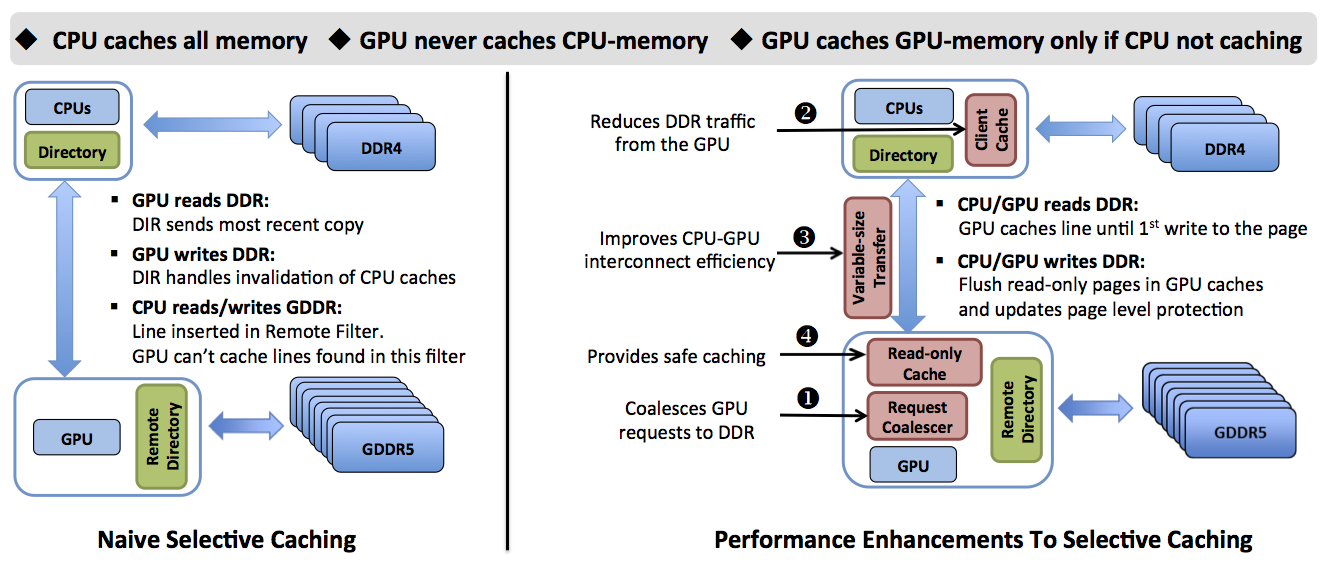
\includegraphics[width=0.9\textwidth]{figures/coherence_overview.png}
% \caption{Overview of naive selective caching implementation and optional performance enhancements.
% Selective caching GPUs maintain memory coherence with the CPU while not
% requiring hardware cache coherence within the GPU domain.}
% \label{fig:coherence_overview}
% % \vspace{.05in}
% \end{figure*}

% \section{Asymmetry Aware GPUs}
% \label{proposal}
% 
% Historically, GPUs have not required hardware cache coherence because their
% programming model did not provide a coherent address space between threads running on separate
% SMs~\cite{CUDA7}.  CPUs however, support hardware cache coherence 
% because it is heavily relied upon by both system and application
% programmers to ensure correctness in multi-threaded programs. 
% Existing GPU programming models do not guarantee data correctness when CPU and GPU accesses
% interleave on the same memory location while the GPU is executing. One way to
% provide such guarantees is to enforce CPU--GPU hardware cache coherence, albeit with significant implementation 
% complexity as previously discussed.
% 
% Alternatively, if the GPU does not cache any data that is concurrently cached by the CPU,
% no hardware coherence messages need to be exchanged between the CPU and GPU, yet data correctness is still guaranteed. 
% This approach also decouples
% the, now private, coherence protocol decisions in CPU and GPU partitions, facilitating multi-vendor 
% system integration.  We now discuss how CPU--GPU
% memory can provide this single shared memory abstraction without implementing 
% hardware cache coherence. We then propose several micro-architectural enhancements to enable selective caching
% to perform nearly as well as hardware cache coherence, while maintaining the programmability benefits of hardware cache coherence.
% 
% \subsection{Naive Selective Caching}
% \label{naiveselectivecaching}
% 
% As shown in Figure~\ref{fig:coherence_overview},
% three simple principles enable the GPU to support a CPU-visible shared memory
% by implementing selective caching. First, the CPU is always allowed to cache any data in the system regardless 
% of whether that data is physically located in the memory attached to the GPU or the CPU\@. 
% Second, the GPU is never allowed to cache data that resides within the 
% CPU memory.  Finally, the GPU may cache data from its 
% own local memory if and only if the CPU is not also caching a copy of this 
% data.
% 
% When the CPU is known to be caching a line that is homed in GPU memory and the GPU requests
% this line, the request must be routed to the CPU where the requested data is serviced 
% from the CPU cache, rather than the GPU memory. Similarly, if the GPU is caching a 
% line that the CPU requests, then this line must be flushed from the GPU caches when the 
% request is received by the GPU memory controller. By dis-allowing caching 
% of memory in use by the CPU, the GPU cannot violate the CPU hardware coherence model.
% 
% The primary microarchitectural structure needed by the GPU to implement
% selective caching is the \emph{remote directory}. The remote directory block
% shown in Figure~\ref{fig:coherence_overview} tracks approximately, but conservatively,
% the cache lines homed in GPU  memory that are presently cached at the CPU.
% When the CPU requests a line from GPU memory,  its cache block address is  
% entered into the remote directory.  If the address was not already present, the GPU
% probes and discards the line from all GPU caches, as in a conventional invalidation-based 
% coherence protocol.  Once a cache block is added to the GPU remote
% directory, it becomes un-cacheable within the GPU; future GPU accesses to the line
% will be serviced from the CPU cache.
% 
% To limit hardware cost, we implement the remote directory as a cuckoo filter 
% (a space efficient version of a counting bloom filter) that never reports
% false negatives but may report false positives~\cite{fan2014,bonomi2006}. Thus, the remote directory may erroneously, but conservatively,
% indicate that a line is cached at the CPU that has never been requested, but will accurately reference
% all lines that have actually been requested.  False positives in the remote directory generate
% a spurious request to the CPU, which must respond with a negative acknowledgement (NACK) should the line
% not be present in the CPU cache.  This request will then be serviced from the GPU memory
% system.  Similarly, if the CPU has cached a line homed in GPU memory (causing a remote directory insertion)
% and has since evicted it, the CPU may also NACK a GPU request, causing the request to return to the GPU memory
% for fulfillment.
% 
% Because entries are inserted but never pruned from our remote directory, we must track if the directory
% becomes full or reaches a pre-selected high-water mark.  If it becomes full, our implementation
% forces the CPU to flush all cache lines homed in GPU memory and then resets the remote directory.  This limited
% cache flush operation  does not flush any lines
% homed in CPU memory, the vast majority of the system's memory capacity.  In our
% design, the flush is performed by triggering a software daemon to call the Linux \texttt{cacheflush} trap.  
% 
% The remote directory is sized to track CPU caching of up to 8MB of GPU memory, which when fully occupied
% requires just 64KB of on-chip storage to achieve a false positive rate of 3\%.  In the workloads we evaluate,
% the remote directory remains largely empty, and neither the capacity nor false positive rate have a significant
% impact on GPU performance.
% If workloads emerge that 
% heavily utilize concurrent CPU--GPU threads, the size and performance of this structure will need to be re-evaluated. 
% However if \texttt{cacheflush} trapping should become excessive due to an undersized remote directory,
% page-migration of CPU--GPU shared pages out of GPU memory and into CPU memory can also be employed to 
% reduce pressure on the GPU remote directory.
% 
% \subsection{Improving Selective Caching Performance}
% \label{microarchimprovements}
% 
% Caches have consistently been shown to provide significant performance 
% gains thanks to improved bandwidth and latency.  As such, naively bypassing the GPU caches based on the mechanisms described in 
% Section~\ref{naiveselectivecaching} should be expected to hurt performance. In this subsection, we describe 
% three architectural improvements that mitigate the impact of selectively bypassing the GPU caches and provide performance approaching
% a system with hardware cache coherence.
% 
% \subsubsection{Cacheless Request Coalescing}
% \label{coalescing}
% 
% The first optimization we make to our naive
% selective caching design is to implement aggressive miss status handling register (MSHR)
% request coalescing for requests sent to CPU memory, labeled \mycirc{1} in Figure~\ref{fig:coherence_overview}.  
% MSHR request coalescing can significantly reduce the request traffic
% to CPU memory without violating coherency guarantees.
% Request coalescing works by promoting
% the granularity of an individual load request (that may be as small as 64 bits)
% to a larger granularity (typically 128B cache lines) before issuing the request
% to the memory system.  While this larger request is in-flight, if other requests
% are made within the same 128B block, then these requests
% can simply be attached to the pending request list in the corresponding MSHR and no new request is issued
% to the memory system.
% 
% To maintain correctness in a selective caching system, this same coalescing
% scheme can be utilized, but data that is returned to the coalesced requests for which no pending
% request is found must be discarded immediately. Discarding data in this way is similar to self-invalidating
% coherence protocols, which attempt to minimize invalidation traffic in CC-NUMA
% systems~\cite{Lebeck95,Lai2000}.  Whereas most MSHR implementations allocate their storage in
% the cache into which the pending request will be inserted, our cache-less request coalescing must have
% local storage to latch the returned data.  This storage overhead is negligible compared to the aggregate
% size of the on-chip caches that are no longer needed with selective caching.
% 
% Table~\ref{tab:coalescing_opportunity} shows the fraction of GPU memory requests 
% that can be coalesced by matching them to pre-existing in-flight memory requests.
% We call request coalescing that happens within a single 
% SM \emph{L1 coalescing} and coalescing across SMs \emph{L1+L2 coalescing}.  
% On average, 35\% of memory requests can be serviced via 
% cacheless request coalescing.  While a 35\% hit rate may seem low when
% compared to conventional CPU caches, we observe that capturing spatial request locality
% via request coalescing provides the majority of the benefit of the L1 caches (44.4\% hit rate) found
% in a hardware cache-coherent GPU, as shown in Table~\ref{tab:gpuhitrate}.
% 
% \begin{table}[tp]
% \begin{center}
% \begin{tabular}{ddd}
%  \hline
%  \multicolumn{1}{l}{Workload}  &  \multicolumn{1}{c}{L1 Coalescing}  &  \multicolumn{1}{c}{L1+L2 Coalescing}  \\
%  \hline
%  \hline
%  \multicolumn{1}{l}{backprop}  &   54.2  &   60.0   \\
%  \hline
%  \multicolumn{1}{l}{bfs}  &   15.8  &   17.6   \\
%  \hline
%  \multicolumn{1}{l}{btree}  &   69.4  &   82.4   \\
%  \hline
%  \multicolumn{1}{l}{cns}  &   24.8  &   28.1   \\
%  \hline
%  \multicolumn{1}{l}{comd}  &   45.7  &   53.8   \\
%  \hline
%  \multicolumn{1}{l}{kmeans}  &   0.0  &   0.0   \\
%  \hline
%  \multicolumn{1}{l}{minife}  &   29.0  &   32.6   \\
%  \hline
%  \multicolumn{1}{l}{mummer}  &   41.9  &   51.1   \\
%  \hline
%  \multicolumn{1}{l}{needle}  &   0.1  &   1.8   \\
%  \hline
%  \multicolumn{1}{l}{pathfinder}  &   41.4  &   45.8   \\
%  \hline
%  \multicolumn{1}{l}{srad\_v1}  &   30.8   &   34.2   \\
%  \hline
%  \multicolumn{1}{l}{xsbench}  &   15.6  &   18.0   \\
%  \hline
%  \hline
%  \multicolumn{1}{l}{Average}  &   30.7  &   35.4  \\
% \hline
% \end{tabular}
% \caption{Percentage of memory accesses that can be coalesced into existing 
% in-flight  memory requests, when using L1 (intra-SM) coalescing, and L1 + L2 (inter-SM) 
% coalescing.}
% \label{tab:coalescing_opportunity}
% \end{center}
% \vspace{-.1in}
% \end{table}
% 
% \subsubsection{CPU-side Client Cache}
% \label{clientcache}
% 
% Although memory request coalescing provides hit rates approaching that of
% conventional GPU L1 caches, it still falls short as it cannot capture
% temporal locality. Selective caching prohibits the GPU from locally caching lines 
% that are potentially shared with the CPU but it does not preclude the GPU from remotely 
% accessing coherent CPU caches.
% We exploit this opportunity to propose a \textit{CPU-side GPU client cache}  (label \mycirc{2} in Figure~\ref{fig:coherence_overview}), which takes 
% advantage of temporal locality not exploited by MSHR coalescing.
% 
% To access CPU memory, the GPU must already send a request to the CPU
% memory controller to access the line. If request coalescing has failed to
% capture re-use of a cache line, then multiple requests for the same line will
% be sent to the CPU memory controller causing superfluous transfers across the DRAM
% pins, wasting precious bandwidth.  To reduce this DRAM pressure, we introduce a small 
% client cache at the CPU memory controller to service
% these GPU requests, thereby shielding the DDR memory system from
% repeated requests for the same line.  Our proposed GPU client cache participates in the 
% CPU coherence protocol much like any other 
% coherent cache on the CPU die, however lines are allocated in this cache only upon 
% request by an off-chip processor, such as the GPU\@.
% 
% This single new cache does not introduce the 
% coherence and interconnect scaling challenges of GPU-side caches,
% but still provides some latency and bandwidth filtering advantages
% for GPU accesses. One might consider an alternative where GPU-requested lines are instead injected into
% the existing last-level cache (LLC) at the CPU.  In contrast to an injection approach, our
% dedicated client cache avoids thrashing the CPU LLC 
% when the GPU streams data from CPU memory (a common access pattern).
% By placing this client cache on the CPU-side rather than the GPU-side of the CPU--GPU 
% interconnect, we decouple the need to extend the CPU's hardware cache coherence protocol into even one on-die GPU cache.
% However, because the GPU client cache is located at the CPU-side of the CPU--GPU interconnect,
% it provides less bandwidth than a GPU-side on-die cache. As described in Section~\ref{background} and 
% shown in Figure~\ref{fig:cache_bw_latency}, this bandwidth loss is typically not performance-critical.
% 
% \subsubsection{Variable-size Link Transfers}
% \label{variablesizing}
% 
% Conventional memory systems access data at cache line granularity to 
% simplify addressing and request matching logic, improve DRAM energy consumption, and 
% exploit spatial locality within caches.  Indeed, the minimum transfer size supported
% by DRAM is usually a cache line.  Cache line-sized transfers work well when data
% that was not immediately needed can be inserted into an on-chip cache, but
% with selective caching, unrequested data transferred from CPU memory must be discarded.  
% Hence, portions of a cache line that
% were transferred, but not matched to any coalesced access, result in wasted
% bandwidth and energy. 
% 
% The effect of this data over-fetch is shown in
% Table~\ref{tab:overfetch}, where cache line utilization is the fraction of the transferred
% line that has a pending request when the GPU receives a cache line-sized response from CPU  memory.
% An average cache line utilization of 60\% indicates that just 77 out of 128 bytes transferred are actually used by
% the GPU\@. 51 additional bytes were transferred across the DRAM interface and CPU--GPU interconnect 
% only to be immediately discarded.
% 
% \begin{table}[tp]
% \begin{center}
% \begin{tabular}{dd}
%  \hline
%  \multicolumn{1}{l}{Workload}  &  \multicolumn{1}{c}{Avg. Cacheline Utilization(\%)}  \\
%  \hline
%  \hline
%  \multicolumn{1}{l}{backprop}  &   85.9  \\
%  \hline
%  \multicolumn{1}{l}{bfs}  &   37.4  \\
%  \hline
%  \multicolumn{1}{l}{btree}  &   78.7  \\
%  \hline
%  \multicolumn{1}{l}{cns}  &   77.6  \\
%  \hline
%  \multicolumn{1}{l}{comd}  &   32.6  \\
%  \hline
%  \multicolumn{1}{l}{kmeans}  &   25.0  \\
%  \hline
%  \multicolumn{1}{l}{minife}  &   91.6  \\
%  \hline
%  \multicolumn{1}{l}{mummer}  &   46.0  \\
%  \hline
%  \multicolumn{1}{l}{needle}  &   39.3  \\
%  \hline
%  \multicolumn{1}{l}{pathfinder}  &   86.6  \\
%  \hline
%  \multicolumn{1}{l}{srad\_v1}  &   96.3  \\
%  \hline
%  \multicolumn{1}{l}{xsbench}  &   30.3  \\
%  \hline
%  \hline
%  \multicolumn{1}{l}{Average}  &   60.6  \\
% \hline
% \end{tabular}
% \caption{Utilization of 128B cache line requests where the returned data 
% must be discarded if there is no matching coalesced request.}
% \label{tab:overfetch}
% \end{center}
% \vspace{-.1in}
% \end{table}
% 
% To address this inefficiency, architects might consider reducing the
% transfer unit for selective caching clients from 128B down to 64 or 32 bytes. While 
% fine-grained transfers improve transfer efficiency by omitting unrequested data, that
% efficiency is offset by the need for multiple small requests and packetization
% overhead on the interconnect. For example, in our link implementation,
% a transfer granularity of 32B achieves at best 66\% link utilization (assuming
% all data is used) due to interconnect protocol overheads, while
% 128B transfers (again, assuming all data is used) can achieve 88\% efficiency.
% 
% To maintain the benefit of request coalescing, but reduce interconnect
% inefficiency, we propose using \textit{variable-size transfer units} on the 
% CPU--GPU interconnect (labeled \mycirc{3} in Figure~\ref{fig:coherence_overview}).  
% To implement variable-size transfer units at the GPU, we allocate GPU MSHR entries at the full
% 128B granularity; coalescing requests as described in Section~\ref{coalescing}.  However, 
% when a request is issued across the CPU--GPU interconnect, we embed a bitmask in the 
% request header indicating which 32B sub-blocks of the 128B cache line should be transferred on the return path.
% While this initial request is pending across the interconnect, if additional requests
% for the same 128B cache line are made by the GPU, those requests will be issued across the interconnect
% and their 32B sub-block mask will be merged in the GPU MSHR.  
% 
% Similar to the GPU-side MSHR, variable sized transfer units require that the CPU-side client cache also maintain pending MSHR
% masks for requests it receives, if it can not service the requests immediately from the
% cache.  By maintaining this mask, when the DRAM returns the 128B line, only those
% 32B blocks that have been requested are transferred to the GPU (again with a bitmask indicating
% which blocks are included).  Because there may be
% both requests and responses in-flight simultaneously for a single 128B line, it is possible
% that two or more responses are required to fulfill the data requested by a single MSHR; the bitmasks
% included in each response facilitate this matching.
% Because GPUs typically perform SIMD lane-level request coalescing within an SM, 32B requests happen 
% to be the minimum and most frequently sized request issued to the GPU memory system.  As a result, we do 
% not investigate supporting link transfer sizes smaller than 32 bytes, which would require microarchitectural
% changes within the GPU SM.
% 
% \subsection{Promiscuous Read-Only Caching}
% \label{readonly}
% 
% Selective caching supports coherence guarantees by bypassing GPU caches when
% hardware cache-coherence operations could be needed.  Thus far, our selective caching architecture
% has assumed that the GPU must avoid caching all data homed in CPU memory.  We identify
% that we can loosen this restriction and allow GPU caching of CPU memory, but only
% if that data can be guaranteed to be read-only by both the CPU and GPU.
% 
% Figure~\ref{fig:readonlymotivation} shows the fraction of data touched by the 
% GPU that is read-only or both read and written, broken down at 
% the OS page (4KB) granularity.  In many workloads, we find the majority 
% of the data touched by the GPU is read-only at the OS page level.  We
% examine this data at page granularity because, even without hardware 
% cache coherence, it is possible (though expensive) to\ignore{ implement coherence}
% guarantee correctness through OS page 
% protection mechanisms entirely in software. 
% Any cache may safely contain data from read-only OS pages.
% However, if the page is re-mapped as read-write, cached copies
% of the data at the GPU must be discarded, which will occur as part
% of the TLB shootdown process triggered by the permission change~\cite{stenstrom1990}.
% 
% \begin{figure}[tp]
% \centering
% 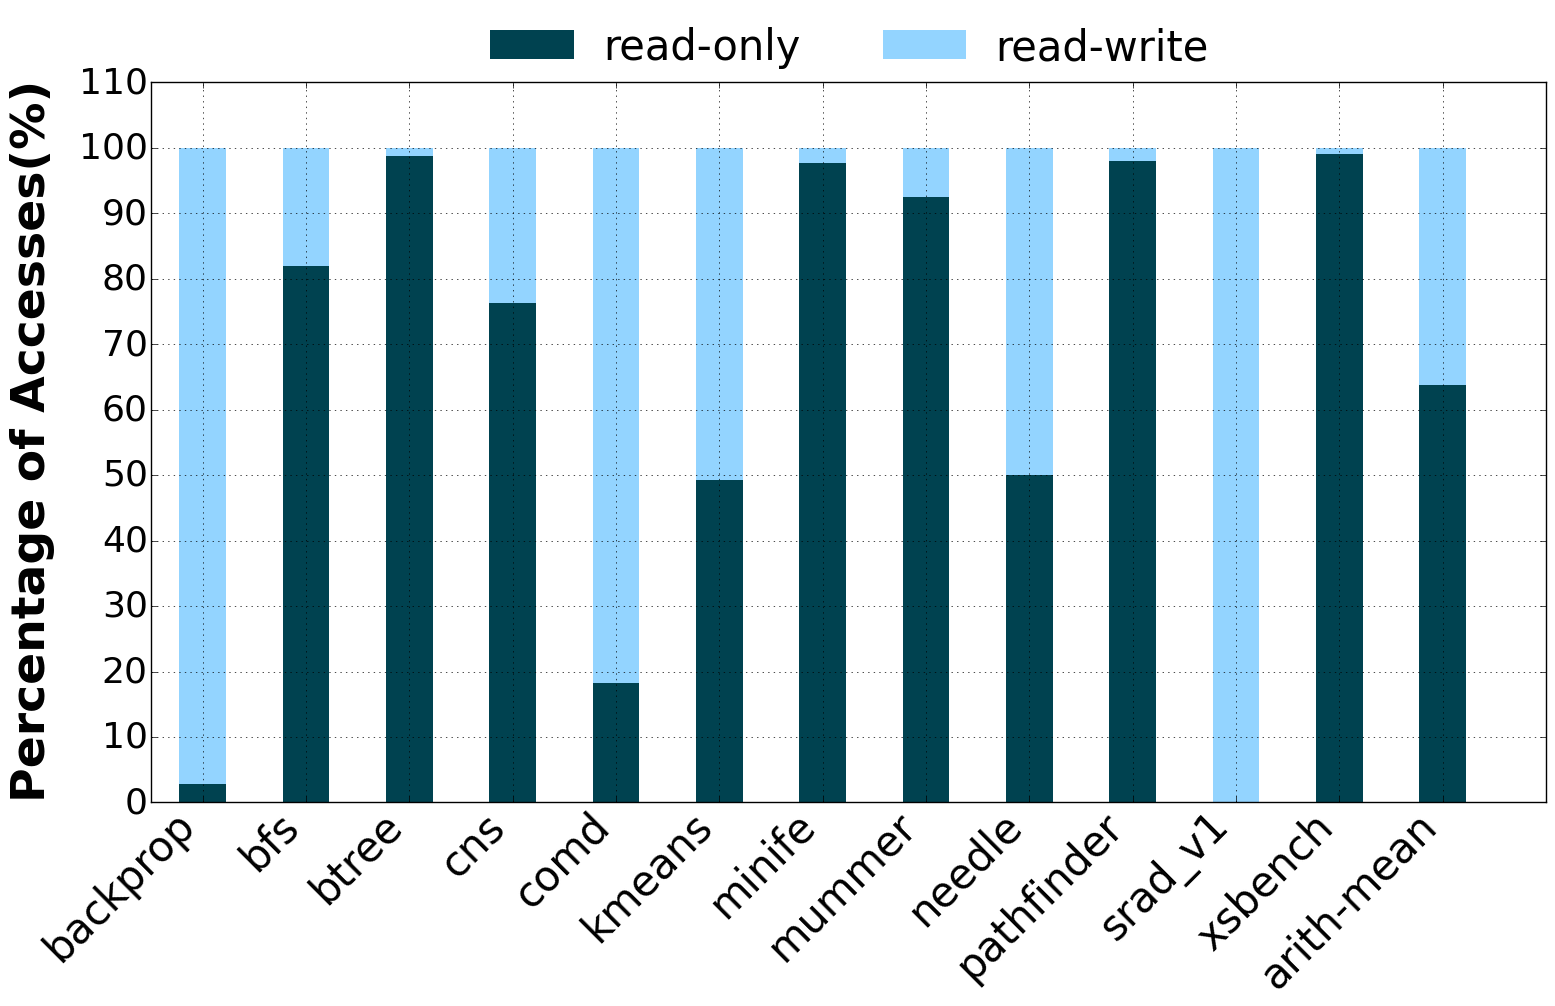
\includegraphics[width=1.0\columnwidth]{figures/read-only.png}
% \caption{Fraction of 4KB OS pages that are read-only and read-write
% during GPU kernel execution.}
% \label{fig:readonlymotivation}
% % \vspace{-.1in}
% \end{figure}
% 
% We propose that despite lacking hardware cache coherence, selective caching GPUs may choose to implement 
% \textit{promiscuous read-only caching of CPU-memory}, relying on such page level software coherence 
% to provide correctness (labeled \mycirc{4} in Figure~\ref{fig:coherence_overview}).  To implement read-only caching, the GPU software 
% run-time system speculatively marks pages within the application as 
% read-only at GPU kernel launch time.  It also tracks which pages may have been marked
% read-only by the application itself to prevent speculation conflicts.  With pages speculatively
% marked as read-only, when the GPU requests pages from the CPU memory, the permissions 
% bit in the TLB entry is checked to determine if lines from this page are cacheable by the 
% GPU\@ despite being homed in CPU memory. Similarly, if the line resides in GPU memory but is marked as cached by
% the CPU in the remote directory, this line can still be cached locally because it is read-only.
% 
% If a write to a read-only page occurs at either the CPU or GPU, a protection
% fault is triggered. A write by the CPU invokes a fault handler
% on the faulting core, which marks the line as read/write at the CPU and
% uncacheable at the GPU.  The fault handler then triggers a TLB shootdown,
% discarding the now stale TLB entry from all CPU and GPU TLBs.
% This protection fault typically incurs a 3-5us delay.  The next access
% to this page at a GPU SM will incur a hardware page walk to refetch this PTE, 
% typically adding < 1us to the first access to this updated page.
% 
% A faulting write at the GPU is somewhat more complex, as protection fault
% handlers currently do not run on a GPU SM.  Instead, the GPU MMU must
% dispatch an interrupt to the CPU to invoke the fault handler.  That SW handler
% then adjusts the permissions and shoots down stale TLB entries, including those at the GPU.
% The CPU interrupt overhead raises the total unloaded latency of the fault to ~20us (as measured
% on NVIDIA's Maxwell generation GPUs). However, only the faulting warp is stalled: the SM can
% continue executing other non-faulting warps.  Once the GPU receives an acknowledgement that the
% fault handling is complete, it will re-execute the write, incurring a TLB miss
% and a hardware page walk to fetch the updated PTE entry.
% 
% The many-threaded nature of the GPU allows us to largely hide 
% the latency of these permission faults by executing other warps, thereby mitigating 
% the performance impact of the high SW fault latency in nearly all of our workloads.
% Nevertheless, software page fault handlers are orders of magnitude more expensive
% than hardware cache-coherence messaging and may erode the benefit of promiscuous 
% read-only caching if permission faults are frequent.  We evaluate the performance of promiscuous 
% caching under different software faulting overhead costs in Section~\ref{readonlyresults}.

\section{Asymmetric Interconnects}
\label{sec:interconnect}

Figure~\ref{fig:symmetric_assymetric}(a) shows a switch connected GPU
with symmetric and static link bandwidth assignment.
Each link consists of equal numbers of uni-directional high-speed
lanes in both directions, collectively comprising a symmetric bi-directional
link. Traditional static-design time link capacity assignment is very common and has
several advantages. For example, only one type of I/O circuitry
(egress drivers or ingress receivers) along with only one type of control logic
are implemented at each on-chip link interface. Moreover, the multi-socket
switches result in simpler designs that can easily support a statically provisioned
bandwidth requirements. On the other hand, multi-socket link bandwidth utilization can have
a large influence on overall system performance. Static partitioning of bandwidth,
when application needs are dynamic, can leave performance on the table.
Because I/O bandwidth is a limited and expensive system resource, NUMA-aware
interconnect designs must look for innovations that can keep wire and I/O
utilization high. 

In multi-socket NUMA GPU systems, we observe that many applications have 
different utilization of egress and ingress channels on both a per GPU-socket basis
and during different phases of execution. For example,
Figure~\ref{fig:link-motivation} shows a link utilization snapshot over time for
\texttt{HPC-HPGMG-UVM} benchmark running on a SW locality-optimized 4-socket NUMA GPU. 
Vertical dotted black lines represent
kernel invocations that are split across the 4 GPU sockets. Several small kernels have
negligible interconnect utilization. However, for the later
larger kernels, GPU0 and GPU2 fully saturate their ingress links,
while GPU1 and GPU3 fully saturate their egress links. At the same time GPU0 
and GPU2, and GPU1 and GPU3 are underutilizing their egress and ingress links respectively.

\begin{figure}[t]
    \centering
    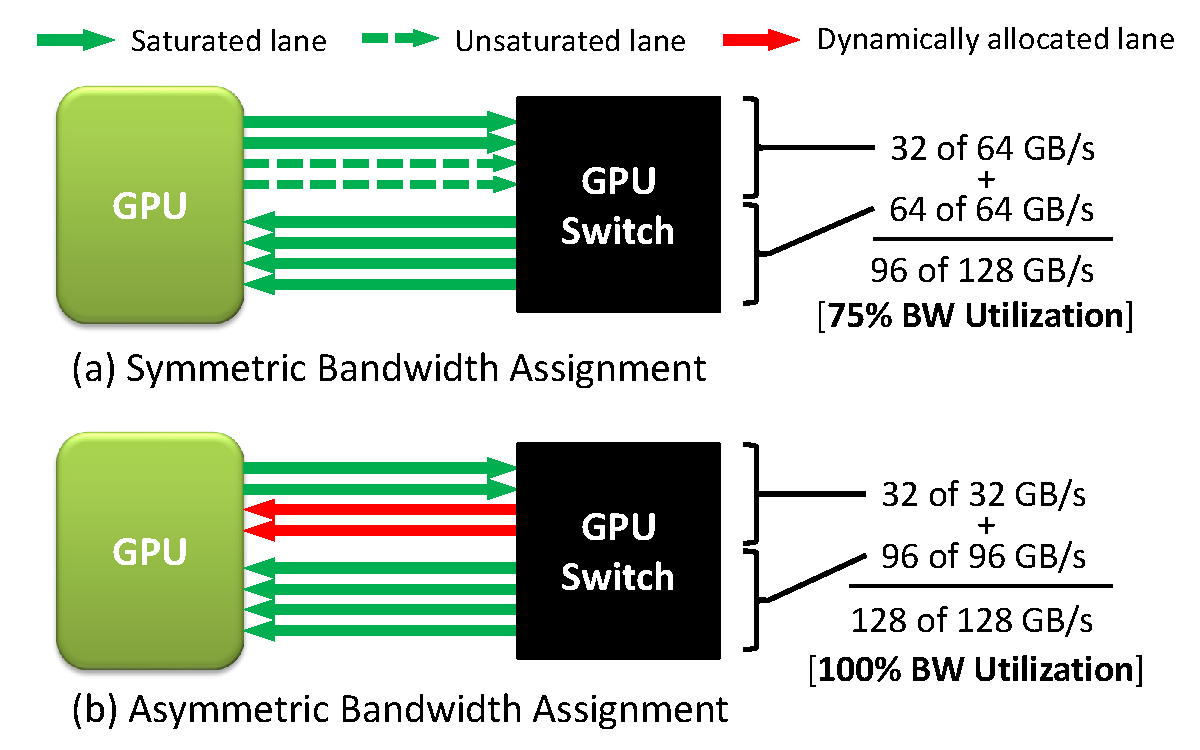
\includegraphics[width=1.0\columnwidth]{figures/link_assignment.pdf}
    \caption{Example of dynamic link assignment to improve interconnect efficiency.}
    \label{fig:symmetric_assymetric}
\end{figure}

In many workloads a common
scenario has CTAs writing to the same memory range at the end of a
kernel (i.e. parallel reductions, data gathering). For CTAs running on one of the
sockets, GPU0 for example, these memory references are local and do not
produce any traffic on the inter-socket interconnections. However CTAs dispatched
to other GPUs must issue remote memory writes, saturating their egress links while
ingress links remain underutilized, but causing ingress traffic on GPU0. 
Such communication patterns typically utilize only
50\% of available interconnect bandwidth. In these cases, dynamically increasing the 
number of ingress lanes for GPU0
(by reversing the direction of egress lanes) and switching the direction of
ingress lanes for GPUs 1--3, can substantially improve the achievable interconnect
bandwidth. Motivated by these findings, we propose to dynamically control multi-socket
link bandwidth assignments on a per-GPU basis, resulting in
dynamic asymmetric link capacity assignments as shown in
Figure~\ref{fig:symmetric_assymetric}(b).  

\begin{figure}[t]
	\centering
	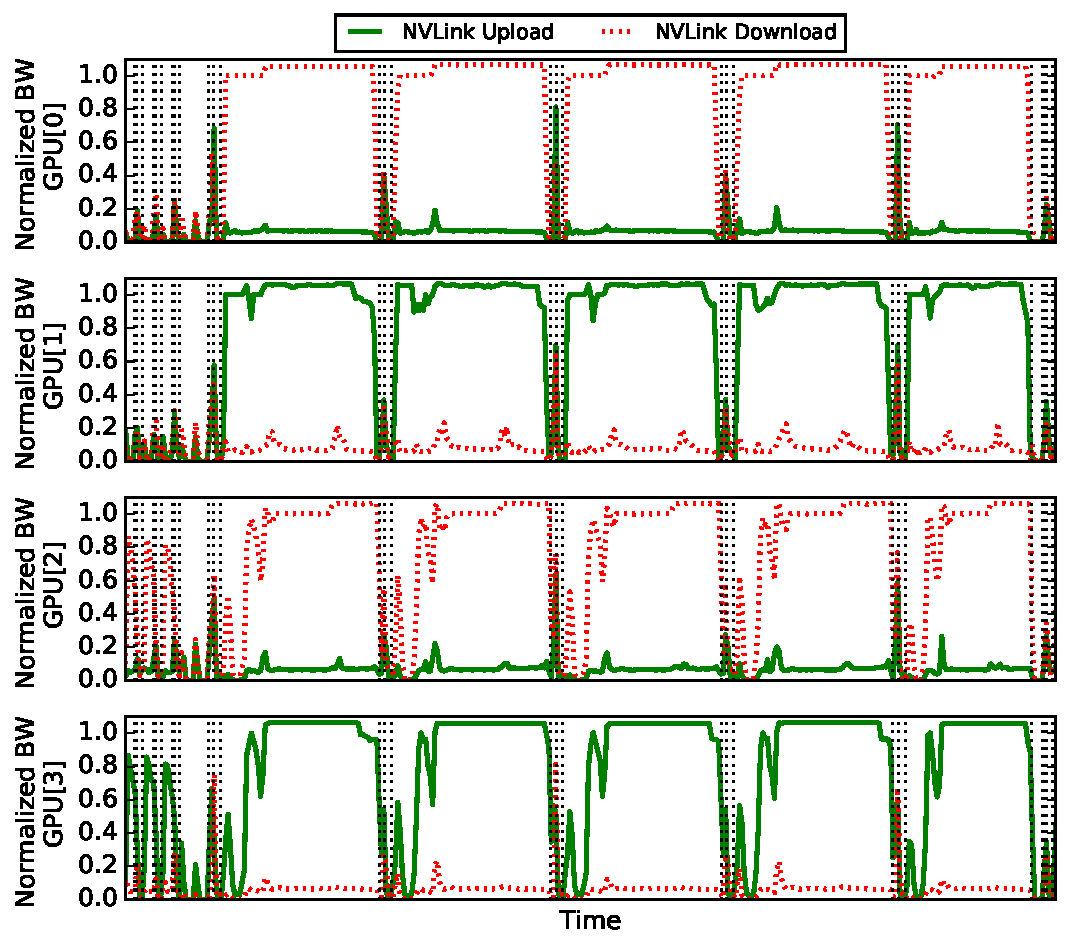
\includegraphics[width=1.0\columnwidth]{figures/bw_profile_HPGMG_UVM_base.pdf}
	\caption{Normalized link bandwidth profile for \texttt{HPC-HPGMG-UVM} 
		showing asymmetric link utilization between GPUs and within a GPU. Vertical black 
		dotted lines indicate kernel launch events.}
	\label{fig:link-motivation}
\end{figure}

To evaluate this proposal, we model point-to-point links containing multiple 
lanes, similar to PCIe~\cite{PCIe3.1a} or NVLink~\cite{pascal-tesla-wp}. In these links, 8 
lanes with \SI{8}{GB/s} capacity per lane yield an aggregate bandwidth of \SI{64}{GB/s} in 
each direction. We propose replacing uni-directional lanes with bi-directional 
lanes to which we apply an adaptive link bandwidth allocation mechanism that 
works as following. For each link in the system, at kernel launch the links are 
always reconfigured to contain symmetric link bandwidth with 8 lanes per 
direction. During kernel execution the link load balancer periodically samples 
the saturation status of each link. If the lanes in one direction are not 
saturated, while the lanes in the opposite direction are 99\% saturated, the 
link load balancer reconfigures and reverses the direction of one of the 
unsaturated lanes after quiescing all packets on that lane. 

\begin{figure*}[tp]
	\centering
	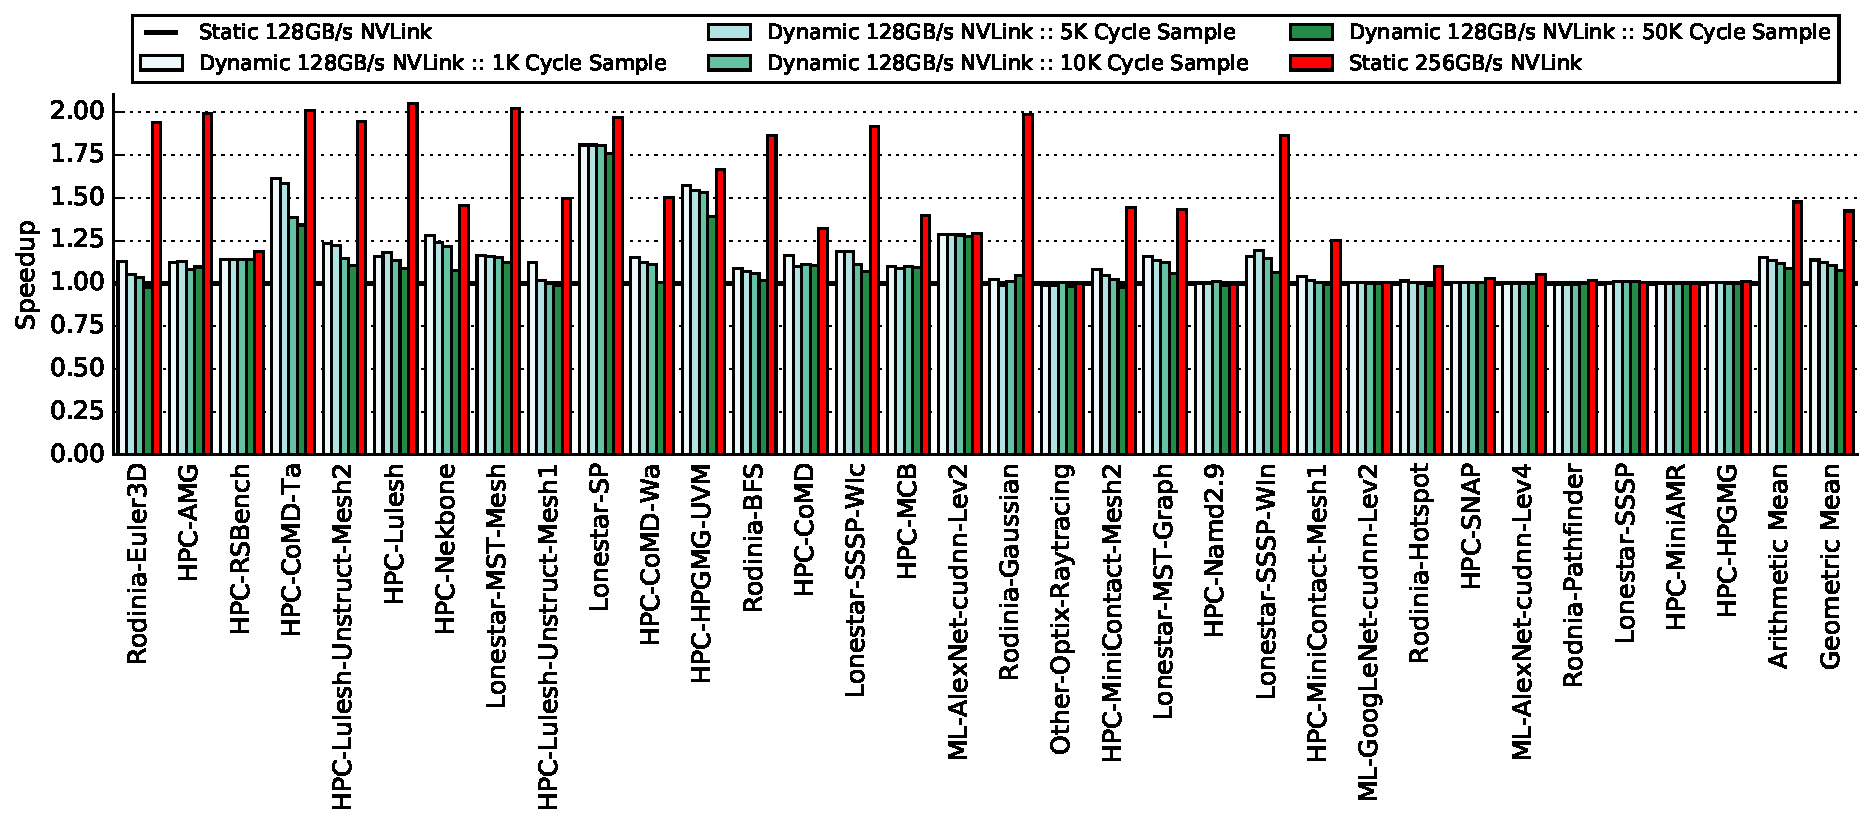
\includegraphics[width=1.0\textwidth]{figures/plot_nvlink_sample_time.pdf}
	\caption{Relative speedup of the dynamic link adaptivity compared to
		the baseline architecture by varying sample time and assuming switch 
		time of
		100 cycles. In red, we also provide speedup achievable by doubling link 
		bandwidth.}
	\label{fig:sampletime}
\end{figure*}

This sample and 
reconfigure process stops only when directional utilization is not 
oversubscribed or all but one lane is configured in a single direction. 
%To avoid instability, we set a threshold between 
%sample intervals corresponding to 5\% of the link bandwidth, below which we do 
%not perform reconfiguration.
If both ingress and egress links are saturated and in an asymmetric 
configuration, links are then reconfigured back toward a symmetric configuration 
to encourage global bandwidth equalization. While this process may sound 
complex, the circuitry for dynamically turning high speed single ended links 
around in just tens of cycles or less is already in use by modern high bandwidth 
memory interfaces, such as GDDR, where the same set of wires is used for both memory reads 
and writes~\cite{hynixgddr51Gb}. In high speed signaling implementations,
necessary phase--delay lock loop
resynchronization can occur while data is inflight; eliminating the need to idle
the link during this long latency (microseconds) operation if upcoming link turn operations
can be sufficiently projected ahead of time, such as on a fixed interval.

\subsection{Results and Discussion} 

Two important parameters affect the performance of
our proposed mechanism: (i)
\texttt{SampleTime} -- the frequency at which the scheme samples for a possible
reconfiguration and (ii) \texttt{SwitchTime} -- the cost of turning the
direction of an individual lane. Figure~\ref{fig:sampletime} shows the 
performance improvement, compared to our locality-optimized GPU by exploring different values of the
\texttt{SampleTime} indicated by green bars and assuming a \texttt{SwitchTime}
of 100 cycles. The red bars in Figure~\ref{fig:sampletime} provide an
upper-bound of performance speedups when doubling the available interconnect
bandwidth to \SI{256}{GB/s}. For workloads on the right of the figure, doubling the link
bandwidth has little effect, indicating that a dynamic link policy will also show little
improvement due to low GPU--GPU interconnect bandwidth demand.
On the left side of the figure, for some
applications when improved interconnect bandwidth has a large effect,
dynamic lane switching can improve application performance by as much as 80\%.
For some benchmarks like \texttt{Rodinia-Euler-3D}, \texttt{HPC-AMG}, and 
\texttt{HPC-Lulesh}, doubling the link bandwidth provides 2$\times$ 
speedup, while our proposed dynamic link assignment mechanism is not 
able to significantly improve performance. These workloads 
saturate both link directions, so there is no opportunity to 
provide additional bandwidth by turning links around.

Using a moderate 5K cycle sample time, the dynamic link policy can improve performance
by 14\% on average over static bandwidth partitioning. If the link load
balancer samples too infrequently, application dynamics can be missed
and performance improvement is reduced. However if the link is reconfigured
too frequently, bandwidth is lost due to the overhead of turning the link.
While we have assumed a pessimistic link turn time of 100 cycles, we performed
sensitivity studies that show even if link turn time were increased to 500
cycles, our dynamic policy loses less than 2\% in performance. 
At the same time, using a faster lane switch (10 cycles) does not
significantly improve the performance over a 100 cycle link turn time.
The link
turnaround times of modern high-speed on-board links such as
GDDR5~\cite{hynixgddr51Gb} are about \SI{8}{ns} with both link and internal 
DRAM turn-around latency, which is less than 10 cycles at \SI{1}{GHz}.

Our results demonstrate that asymmetric link bandwidth
allocation can be very attractive when inter-socket interconnect bandwidth is constrained 
by the number of on-PCB wires (and thus total link bandwidth).
The primary drawback of this solution is that both types of interface circuitry (TX and RX)
and logic must be implemented for each lane in both the GPU and switch interfaces.
We conducted an analysis of the potential cost of doubling the amount
of I/O circuitry and logic based on a proprietary state of
the art GPU I/O implementation. Our results show that doubling this interface area
increases total GPU area by less than 1\% while yielding a 12\% improvement in average
interconnect bandwidth and a 14\% application performance improvement.  
One additional caveat worth noting is that the proposed asymmetric link
mechanism optimizes link bandwidth in a given direction for each individual
link, while the total switch bandwidth remains constant.
%This means that potential improvement is subject to per-link imbalance and cannot improve
%situations where there is large global bandwidth imbalance occurring.
 

% DO NOT REMOVE, we can use this to compute POWER later 
%from http://teams.nvidia.com/sites/Corporate/ntech/SiteAssets/downloads/2014/NTECH2014_SlideDecks20(presented)/7.1_Osborn.pptx 
%Power: 8 lanes (TX + RX) at 25GT/s ~= 1.5W 
%Area: 8 Lane PHY (8 TX + 8 RX + PLL) ~= 3.3mm^2 
%Physical Data: 7.5pJ/b transferred




\section{NUMA-Aware Cache Management}
\label{sec:caches}
In Section~\ref{sec:interconnect} we have shown that inter-socket bandwidth is an
important factor in achieving scalable NUMA GPU performance.
Unfortunately, because either the outgoing or incoming links must be underutilized
for us to reallocate that bandwidth to the saturated link, if both incoming and
outgoing links are saturated, dynamic link rebalancing yields minimal gains.
To improve performance in situations where dynamic link balancing is ineffective,
system designers can either increase link bandwidth, which is very expensive,
or try and decrease the amount of traffic that crosses the low bandwidth
communication channels.  To decrease off-chip memory traffic, architects typically
turn to caches to capture locality.

\begin{figure*}[t]
    \centering
    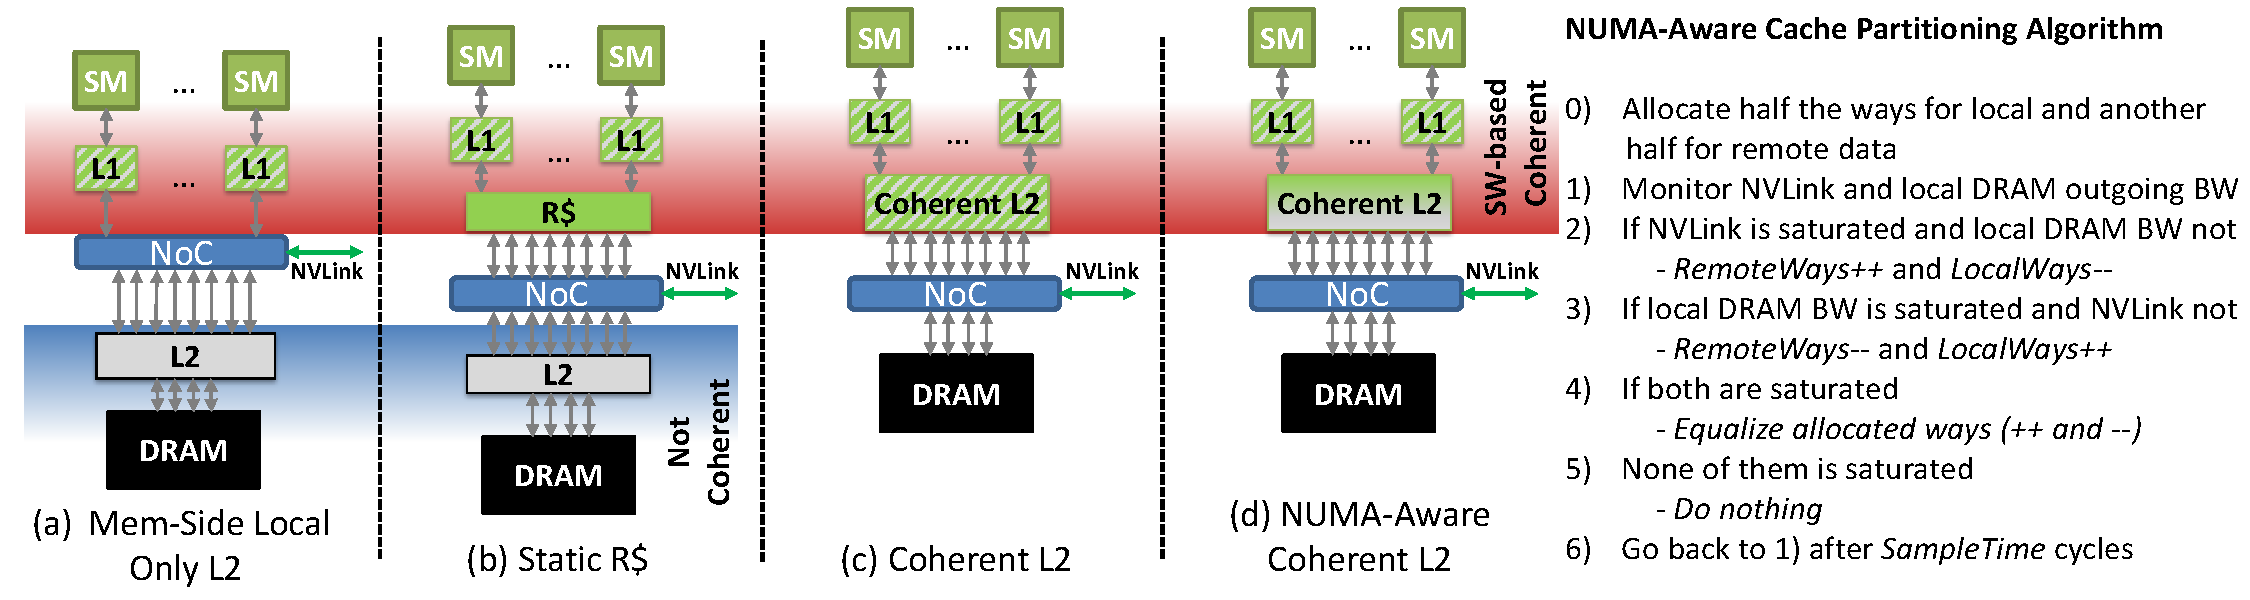
\includegraphics[width=1.0\textwidth]{figures/cache_configurations_static_dynamic.pdf}
    \caption{Potential L2 cache organizations to balance capacity between remote and
    local NUMA memory systems.}
    \label{fig:cacheorg}
            \vspace{-.2in}
\end{figure*}

GPU cache hierarchies differ from traditional CPU hierarchies where in they 
are not supported by strong hardware coherence protocols~\cite{singh2013cache}. 
They also differ from CPU protocols in that caches may be both processor side 
(where some form of 
coherence is typically necessary) or they may be memory side (where coherence 
is not necessary).  As described in Table~\ref{tab:setup} and
Figure~\ref{fig:cacheorg}(a), a GPU today is typically composed of relatively 
large SW managed coherent L1 caches located close to the SMs, while a relatively small, 
distributed, 
non-coherent memory side L2 cache resides close to the memory controllers.  
This organization works well for GPUs 
because their SIMT processor designs often allow for significant coalescing 
of requests to the same cache line, so having large L1 caches reduces the 
need for global crossbar bandwidth.  By then placing the L2 caches 
memory-side they do not need to participate in the coherence protocol, reducing
complexity.

\subsection{Design Considerations}
In NUMA designs remote memory references occurring across low bandwidth NUMA 
interconnections results in poor performance, as shown in 
Figure~\ref{fig:motivation}. Similarly, in NUMA GPUs utilizing
traditional memory side L2 caches (that depend on fine grained memory 
interleaving for load balancing) is a bad decision. Because memory side caches only
able to cache accesses that originate in their local memory-side, they cannot
cache memory from other NUMA zones and thus can not reduce NUMA interconnect traffic.  
Previous work has proposed that GPU L2 cache capacity should be split between 
memory-side caches and a new processor-side L1.5 cache that is an extension 
of the GPU L1 caches~\cite{Arunkumar2017} to enable caching of remote data, shown
in Figure~\ref{fig:cacheorg}(b). By balancing L2 capacity between memory side 
and remote caches (R\$), this design limits the need for extending expensive coherence
operations (invalidations) into the entire L2 cache while still 
minimizing crossbar or interconnect bandwidth.

\textbf{Flexibility:} Designs that statically allocate cache capacity to local memory and remote memory, 
in any balance, may achieve reasonable performance in specific instances 
but they lack flexibility. Much like application phasing was shown to affect 
NUMA bandwidth consumption the ability to dynamically share cache capacity between local and 
remote memory has the potential to improve performance under several 
situations. First, when application phasing results in some GPU-sockets
primarily accessing data locally while others are accessing data remotely,
a fix partitioning of cache capacity is guaranteed to be sub-optimal.
Second, while 
we show that most applications will be able to completely fill large 
NUMA GPUs, this may not always be the case. GPUs within the data center are 
being virtualized and there is on-going work to support concurrent execution 
of multiple \hl{processes} within a single GPU~\cite{park2015chimera, 
lin2016enabling,puthoor2016implementing,HSATASKMODEL}. If a large NUMA GPU is sub-partitioned, it is intuitive 
that system software attempt to partition it along the NUMA boundaries (even within
a single GPU-socket) to improve the locality of small GPU kernels.
To effectively  capture locality in these situation, NUMA-aware GPUs need to be able to 
dynamically re-purpose cache capacity at runtime, rather than be statically partitioned at design time. 

\textbf{Coherence:} To-date, \hl{discrete}
single socket GPUs have not moved their memory-side caches to processor side 
because the overhead of cache invalidation (due to coherence) is an 
unnecessary performance penalty.  Within a single socket GPU with a uniform
memory system, there is little performance advantage to implementing L2 caches
as processor side caches.  However in a multi-socket NUMA design, the performance tax
of extending coherence into L2 caches is offset by the fact that remote memory
accesses can now be cached locally and may be justified;
Figure~\ref{fig:cacheorg}(c) shows a configuration with 
a coherent L2 cache where remote and local data contend for L2 capacity as
extensions of the L1 caches, implementing identical coherence policy.

\textbf{Dynamic Partitioning:} Building upon coherent GPU L2 caches, we posit that while 
conceptually simple, allowing both remote and 
local memory accesses to contend for cache capacity (in both the L1 and L2 caches) 
in a NUMA system is flawed. In UMA systems it is well know that performance 
is maximized by optimizing for cache 
hit rate, thus minimizing off-chip memory system bandwidth. However in NUMA systems, 
\textit{not all cache misses have the same relative cost
performance impact}. A cache miss to a local memory address has a 
smaller cost (in both terms of latency and bandwidth) than a cache miss to a 
remote memory address. Thus, it should be beneficial to dynamically 
skew cache allocation to preference caching remote memory over 
local data when it is determined the system is bottle-necked on NUMA bandwidth.

\begin{figure*}[t]
    \centering
    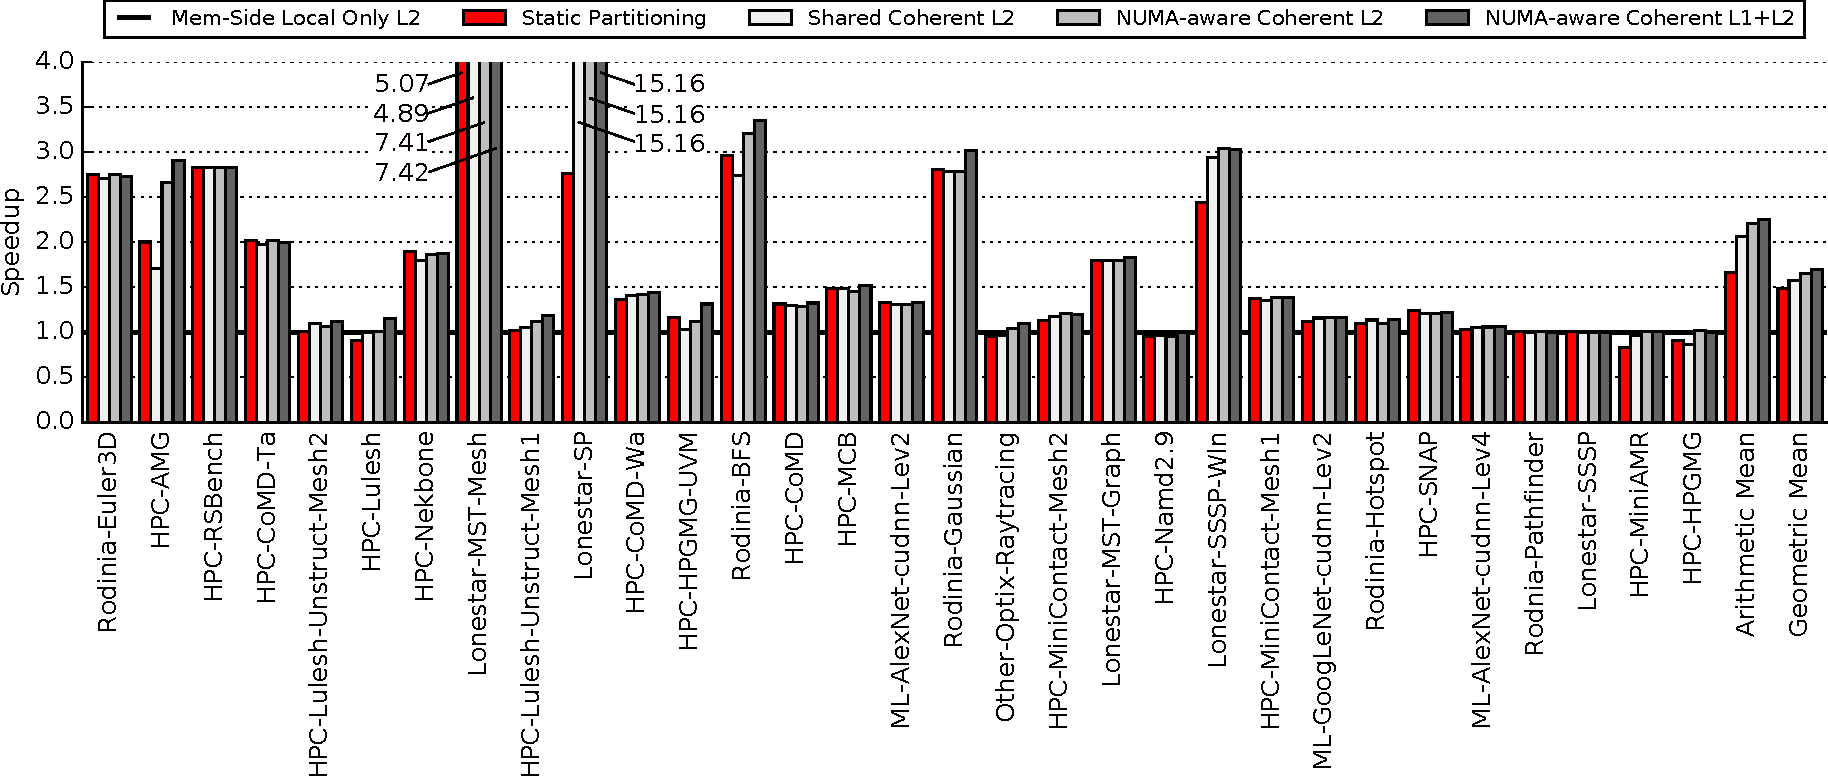
\includegraphics[width=1.0\textwidth]{figures/plot_merged_cache_WB.pdf}
    \caption{Performance of NUMA-aware dynamic cache partitioning in a 4-socket
	GPU compared to memory-side L2 and previously proposed static partitioning.}
    \label{fig:dynamiccaching}
        \vspace{-.2in}
\end{figure*}

\begin{figure}[t]
    \centering
    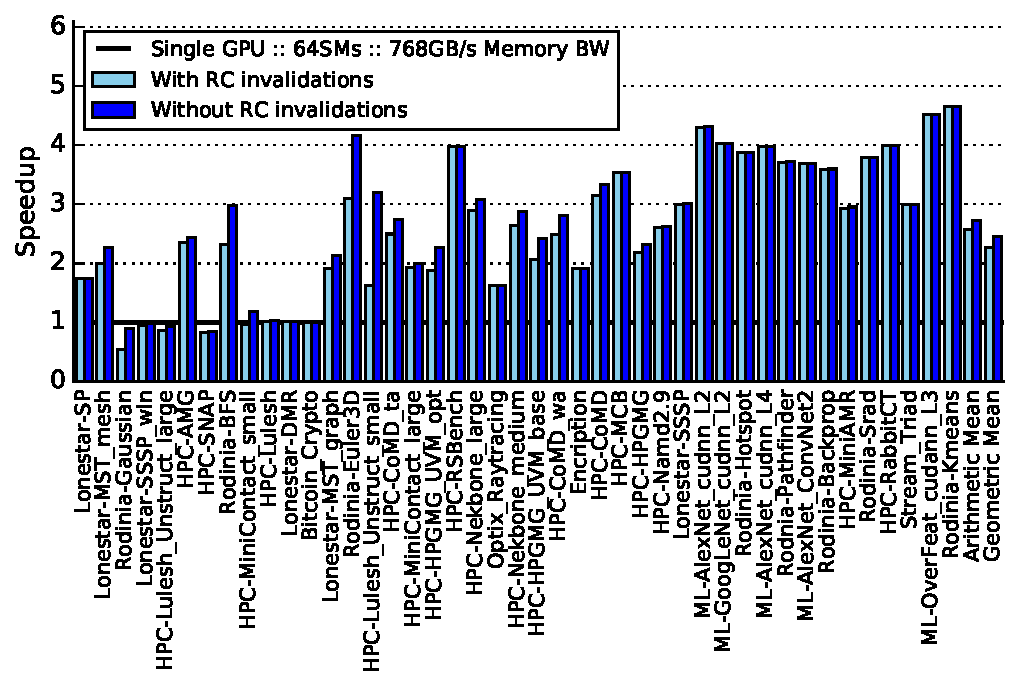
\includegraphics[width=1.0\columnwidth]{figures/plot_no_inval_WB.pdf}
    \caption{Performance overhead of extending current GPU software based coherence
    into the GPU L2 caches.}
    \label{fig:invalidations}
    \vspace{-.2in}
\end{figure}


To minimize inter-GPU bandwidth in multi-socket GPU systems we propose a
NUMA-aware cache partitioning algorithm, with cache organization and brief summary 
shown in Figure~\ref{fig:cacheorg}(d).  Similar to our interconnect balancing
algorithm, at initial kernel launch (after GPU caches have been flushed for
coherence purposes) we allocate one half of the cache ways for local memory and 
the remaining ways for remote data (Step \circled{0}). After executing for a 5K cycles 
period, we sample the average bandwidth utilization on local memory and estimate
the GPU-socket's incoming read request rate by looking at the outgoing request rate
multiplied by the response packet size.  By using the outgoing request rate to estimate
the incoming bandwidth, we avoid situations where incoming writes may saturate
our link bandwidth falsely indicating we should preference remote data caching.
Projected link utilization above 99\% is considered to be bandwidth saturated 
(Step \circled{1}). In cases where the interconnect bandwidth is saturated but
local memory bandwidth is not, the partitioning algorithm attempts to reduce remote 
memory traffic by re-assigning one way from the group of local ways to the
remote ways grouping (Step \circled{2}).
Similarly, if the local memory BW is saturated and NVLink is not, the policy 
re-allocates one way from the remote group, and allocates it to the group of local ways (Step 
\circled{3}).  To minimize the impact on cache design, all ways are consulted on look
up, allowing lazy eviction of data when the way partitioning changes.
In case where both the interconnect and local memory bandwidth 
are saturated, our policy gradually equalizes the number of ways assigned for remote 
and local cache lines (Step \circled{4}). Finally, if neither of the links are 
currently saturated, the policy takes no action (Step \circled{5}).  To prevent
cache starvation of either local or remote memory (which causes memory latency
dramatically increase and a subsequent drop in performance), we always require at 
least one way in all caches to be allocated to either remote of local memory.

\begin{figure*}[tp]
    \centering
    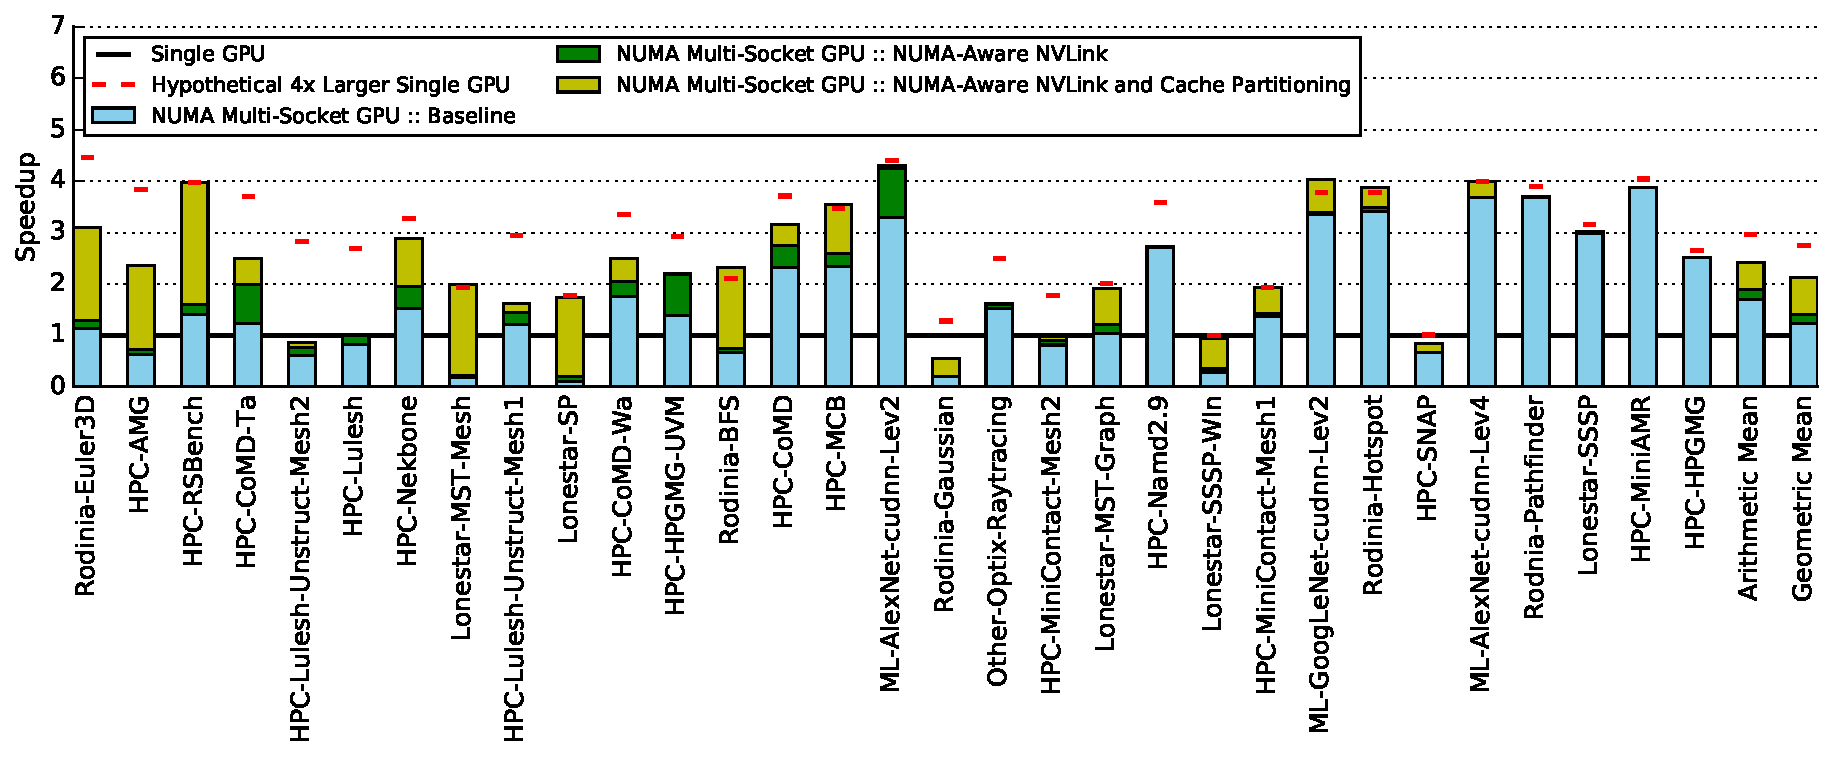
\includegraphics[width=1.0\textwidth]{figures/plot_final_speedup_WB_nvlink_first.pdf}
    \caption{Final NUMA-aware GPU performance compared to a single GPU and 4$\times$ larger single GPU with scaled resources.}
    \label{fig:combined}
    \vspace{-.2in}
\end{figure*}

\subsection{Results}

Figure~\ref{fig:dynamiccaching} compares the performance of 4 different cache
configurations in our 4-socket NUMA GPU. Our baseline is a traditional
GPU with memory side local-only L2 caches. To compare against prior work~\cite{Arunkumar2017} we
provide a 50--50 static partitioning where the L2 cache budget is split between the 
GPU-side coherent remote cache which contains only 
remote data, and the memory side L2 which contains only local data. In our 4-socket NUMA
GPU static partitioning improves performance by 54\% on average, although for some benchmarks, 
it hurts the performance by as much as 10\% for workloads that have negligible
inter-socket memory traffic. We also show the results for GPU-side
coherent L1 and L2 caches where both local and remote data contend capacity.
On average, this solution outperforms static cache partitioning significantly
despite incurring additional flushing overhead due to cache coherence.

Finally, our proposed NUMA-aware cache 
partitioning policy is shown in dark grey. Due to its ability to
dynamically adapt the capacity of both L2 and L1 to optimize performance when backed
by NUMA memory, it is the highest performing cache configuration. By examining
simulation results we find that for workloads on the left side of Figure~\ref{fig:dynamiccaching} 
which fully saturate the NVLink bandwidth, NUMA-aware dynamic policy configures the L1 and 
L2 caches to be primarily used as remote caches.  However, workloads on the right 
side of the figure tend to have good GPU-socket memory locality, and thus 
prefer L1 and L2 caches store primarily local data.  NUMA-aware cache
partitioning is able to flexibly adapt to varying memory access profiles and
can improve average NUMA GPU performance 76\% compared to traditional memory side L2
caches, and 22\% compared to previously proposed static cache partitioning despite
incurring additional coherence overhead.

\hl{\textbf{Coherence Invalidation Overheads:} When extending the software controlled GPU coherence protocol into the GPU L2 
caches, L1 coherence operations (flushes) must also be extended into the GPU 
L2 caches. Using bulk software invalidation to maintain coherence is simple to
implement in hardware but risks having significant performance penalty when evicting
data from caches that is not required to maintain correctness.  The impact of this bulk
invalidation is dependant on both the frequency of the invalidations as well as the scope
(cache capacity) effected.  While GPU vendors like NVIDIA have chosen to implement software
controlled invalidate at the L1 level, extending these invalidations to the L2 (and across
multiple GPUs) increases both the capacity and frequency of the invalidation events that
occur.}

\hl{To understand the impact these additional coherence operations have on our 
NUMA-aware cache performance, we evaluate a hypothetical L2 cache which ignores the cache 
invalidation events, thus representing
the upper limit on performance (no coherence evictions ever occur) that could be achieved, 
even using a fine grain coherence protocol.}
Figure~\ref{fig:invalidations} shows the impact that coherence
operations have on application performance in our 4-socket NUMA GPU.  While significant for
some applications, on average SW based GPU coherence overheads are only 10\% even
when extended into all GPU-socket L2 caches; \hl{we conclude that despite
the coherence overheads the benefit of NUMA-aware coherent L2 caches on 
multi-socket GPUs is a worthy trade-off for GPU workloads that do not yet rely
on significant fine grain synchronization between GPUs or GPUs and CPUs.}





\section {Discussion}

\label{discussion}
\begin{figure*}[tp]
    \centering
    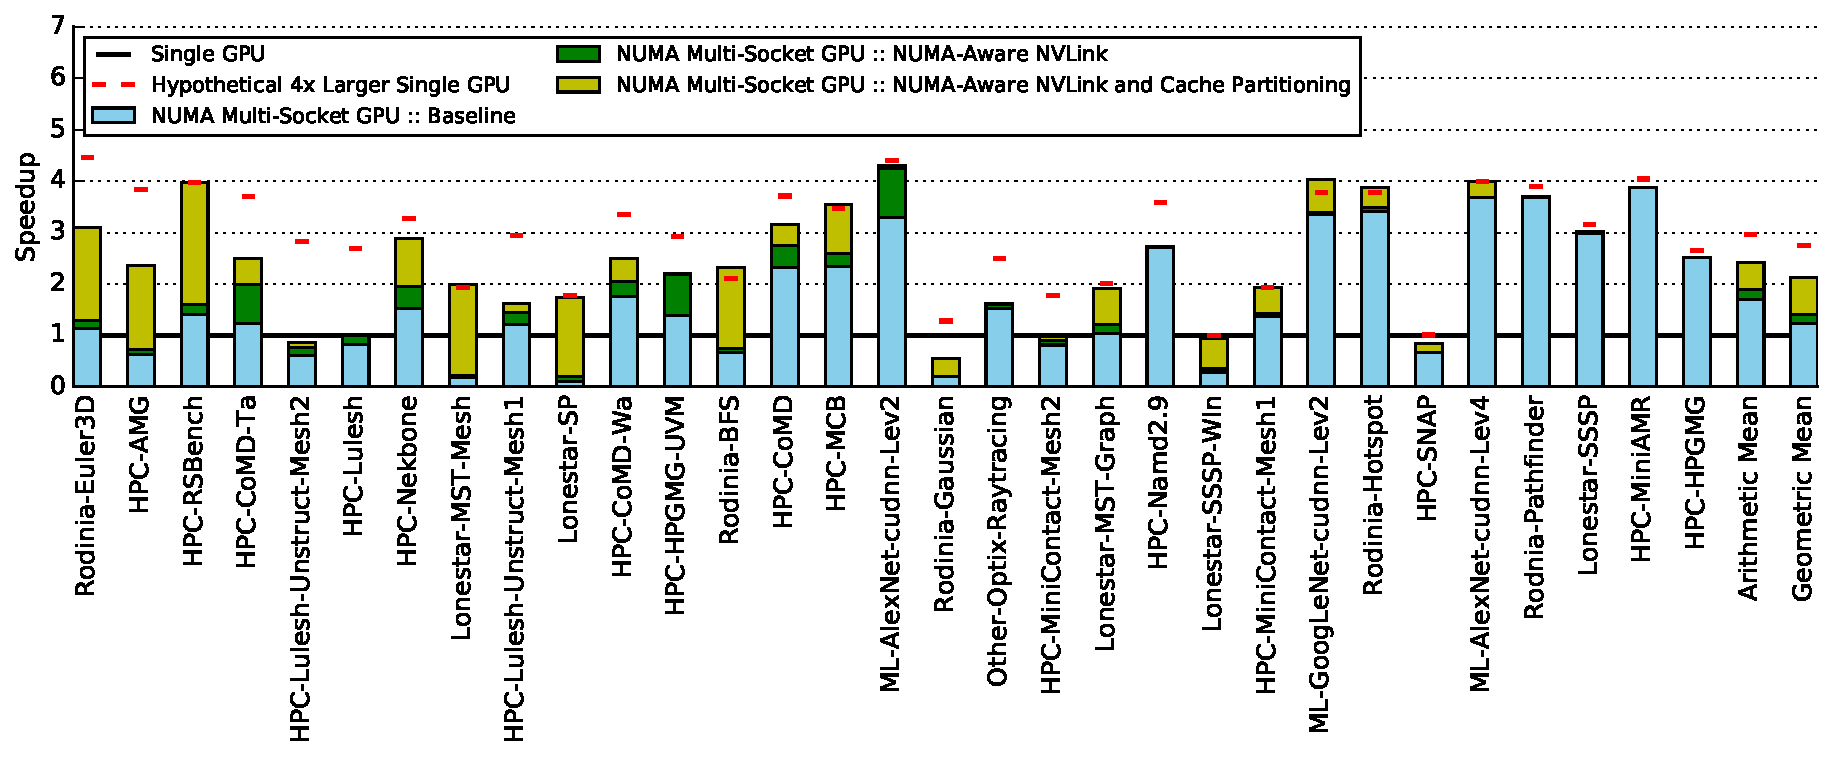
\includegraphics[width=0.9\textwidth]{figures/plot_final_speedup_WB_nvlink_first.pdf}
    \caption{Performance of multi-socket GPU with combined assymetric 
optimizations.}
    \label{fig:combined}
\end{figure*}

In Sections~\ref{interconnect} and~\ref{caching} we explored the performance 
implications of dynamically managing GPU interconnect bandwidth and allowing 
individual GPUs to dymnamically allocate on-chip cache capacity to decrease 
dependance on memory system resources when oversubscribed.  Both of these 
techniques aim to more efficiently utilize the available system bandwidth within 
our NUMA multi-GPU system, closing the gap between multi-socket bandwidth and 
local memory bandwidth.  These two techniques are orthoginal and could be 
applied in isolation or in combination.  Dynamic interconnect balancing has an 
implementation advantage in that the system level changes to enable this feature 
are very isolated from the larger GPU, only the link level load balancer on both 
the GPU and switch need to be modified.  Conversely, enabling GPU caching of 
remote memory and dynamic balancing of cache capacity based on interconnect 
utilization requires changes to both the physical cache architectures and the 
GPU coherence protocol.

Because these two features target similar improvements, when employed together 
their effects are not strictly additive.  Figure~\ref{fig:combined} shows the 
improvement when applying both dynamic interconnect and dynamic cache management 
together.  For benchmarks such as \texttt{CoMD}, these features contribute 
nearly equally to the overall improvement, but for others such as 
\texttt{HPGMG} or \texttt{MST}, interconnect improvements or caching are the 
primary contributor respectively.  On average, we observe that when combined we 
see XXX\% improvement in multi-GPU performance when applying our proposed 
optimizations.

\begin{figure*}[t]
    \centering
    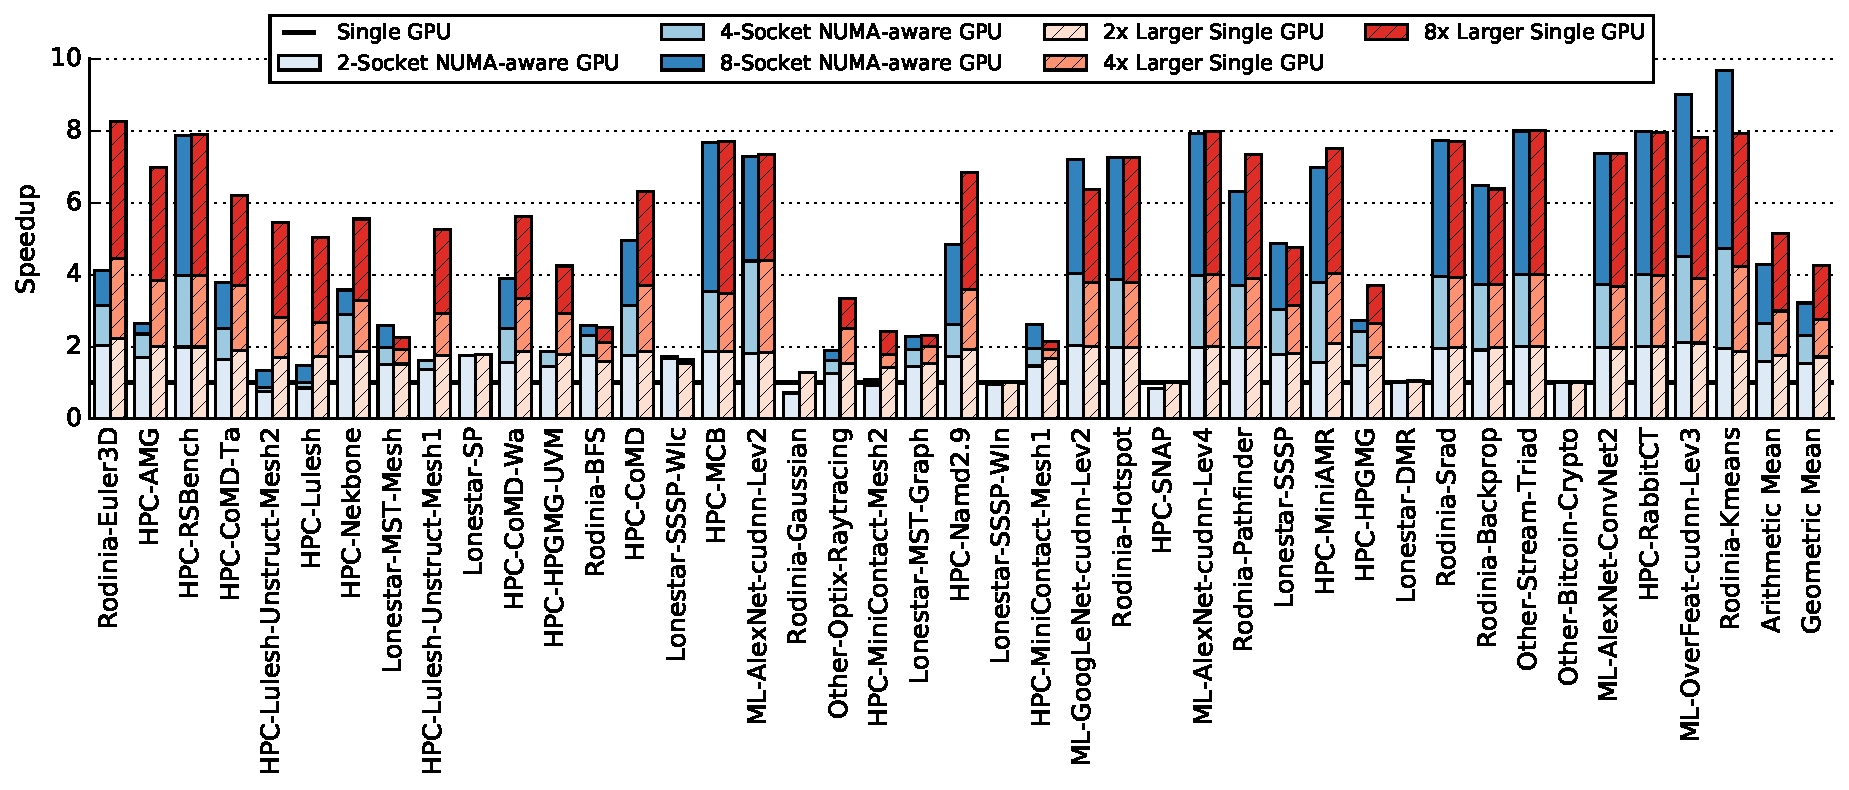
\includegraphics[width=1.0\textwidth]{figures/plot_scalability_mgpu_WB.pdf}
    \caption{Scalability of multi-socket GPU as we move from 1-8 GPUs}
    \label{fig:scalability}
\end{figure*}

\textbf{Scalability:} When considering moving from a single socket GPU to
multi-socket GPU solutions the question arises of what level of efficiency
can be maintained with this approach.  Figure~\ref{fig:scalability} shows the
scalability of a multi-socket GPU approach as we move from a single to 
eight socket multi-GPU implementation.  While larger multi-socket GPUs
may be possible to power and cool within a single node, we observe that due
to parallel efficiency XXX, XXX, XXX.

Another paragraph here once we have results.\vspace{1in}

\textbf{Multi-Tenancy of Large GPUs:} In this work we have shown that many 
workloads today have the ability to
saturate (with sufficient parallel work) a GPU that is at least 4$\times$
larger than today's GPUs.  With deep data becoming commonplace across many
computing paradigms, we believe that the trend of having enough computation
to saturate much larger single GPUs will continue into the forseeable future.
However, when GPUs become larger at the expense of having multiple discrete
GPUs within the system, questions related to GPU provisioning arise.  Applications
that cannot saturate such a GPU will leave resources underutilized and applications
that may be running concurrently in the system currently have to coarse grain
multi-plex the GPU in time cooperatively.  

While not the focus of this work,
there is significant effort in both industry and academia to support finer
grain sharing of GPUs through either shared SM execution~\cite{XXX}, spatial
multi-plexing of a GPU~\cite{XXX}, or through improved time division multiplexing
with GPU pre-emptability~\cite{XXX}.  To support improved per GPU efficiency,
any of these solutions could be applied to a multi-socket GPU to improve utilization
in cases where applications can not fill a significantly larger GPU.  Alternatively,
with additional software work multi-socket GPU designs should be able to be dynamically
partitioned with granularity from 1--N logical GPUs if they are switch connected, providing
yet another level of partitionable flexibility.

\textbf{Power Implications:} \textit{Oreste or Evgeny}
What happens to all the extra bandwidth we need over the interconnect and
power.  we should calculate the extra power but note that even using P2P GPU
access there will still be many remote accesses.  unfortunately we can't quantify
that differential because (drives the point home) there are not multi-GPU versions
for most of our 40+ benchmarks.

% 
% % 
% % One use case in the future
% % may be that GPU programmers will size their application's data to extend well 
% beyond
% % the performance-optimal footprint in CPU and GPU memory.  With excess data 
% spilling over
% % into the additional capacity provided by the CPU memory, performance
% % bottlenecks will shift away from the GPU towards the CPU memory system.  In 
% such
% % cases, the GPU caching policy for CPU memory will come under additional 
% pressure due to
% % the increased traffic skewed towards CPU memory.
% % 
% % To understand how selective caching affects performance under such a scenario, 
% we evaluate
% % a situation wherein the application data has been
% % sized so that 90\% of the footprint resides in CPU memory and just 10\% can 
% fit within GPU memory, as compared to the nearly
% % inverse performance-optimal 20\%-80\% ratio.
% % Figure~\ref{fig:capacityconstrained} shows the performance of this 
% memory-capacity-constrained case relative 
% % to the baseline optimal ratio.  We see that naive selective caching and
% % our proposed enhancements follow the same trend of performance improvements
% % shown previously in Section~\ref{results}.  Because this scenario is primarily 
% limited
% % by the CPU memory system, we see that in some cases the client cache and 
% variable sized transfer interconnect optimizations
% % can actually outperform the hardware cache-coherent GPU due to a reduction in 
% data overfetch between the CPU memory and the GPU client.
% % To validate our observation, we added the same client cache and variable
% % transfers to the hardware cache-coherent baseline configuration and saw an 
% average
% % speedup of 4.5\%.  Whereas the absolute
% % performance achieved, compared to a performance-optimal memory footprint and 
% allocation, may not always be compelling, should
% % software designers chose to partition their problems in this way, we believe 
% selective caching will continue to 
% % perform as well as a hardware cache-coherent GPU.
% % 
% % \begin{figure}[t]
% % 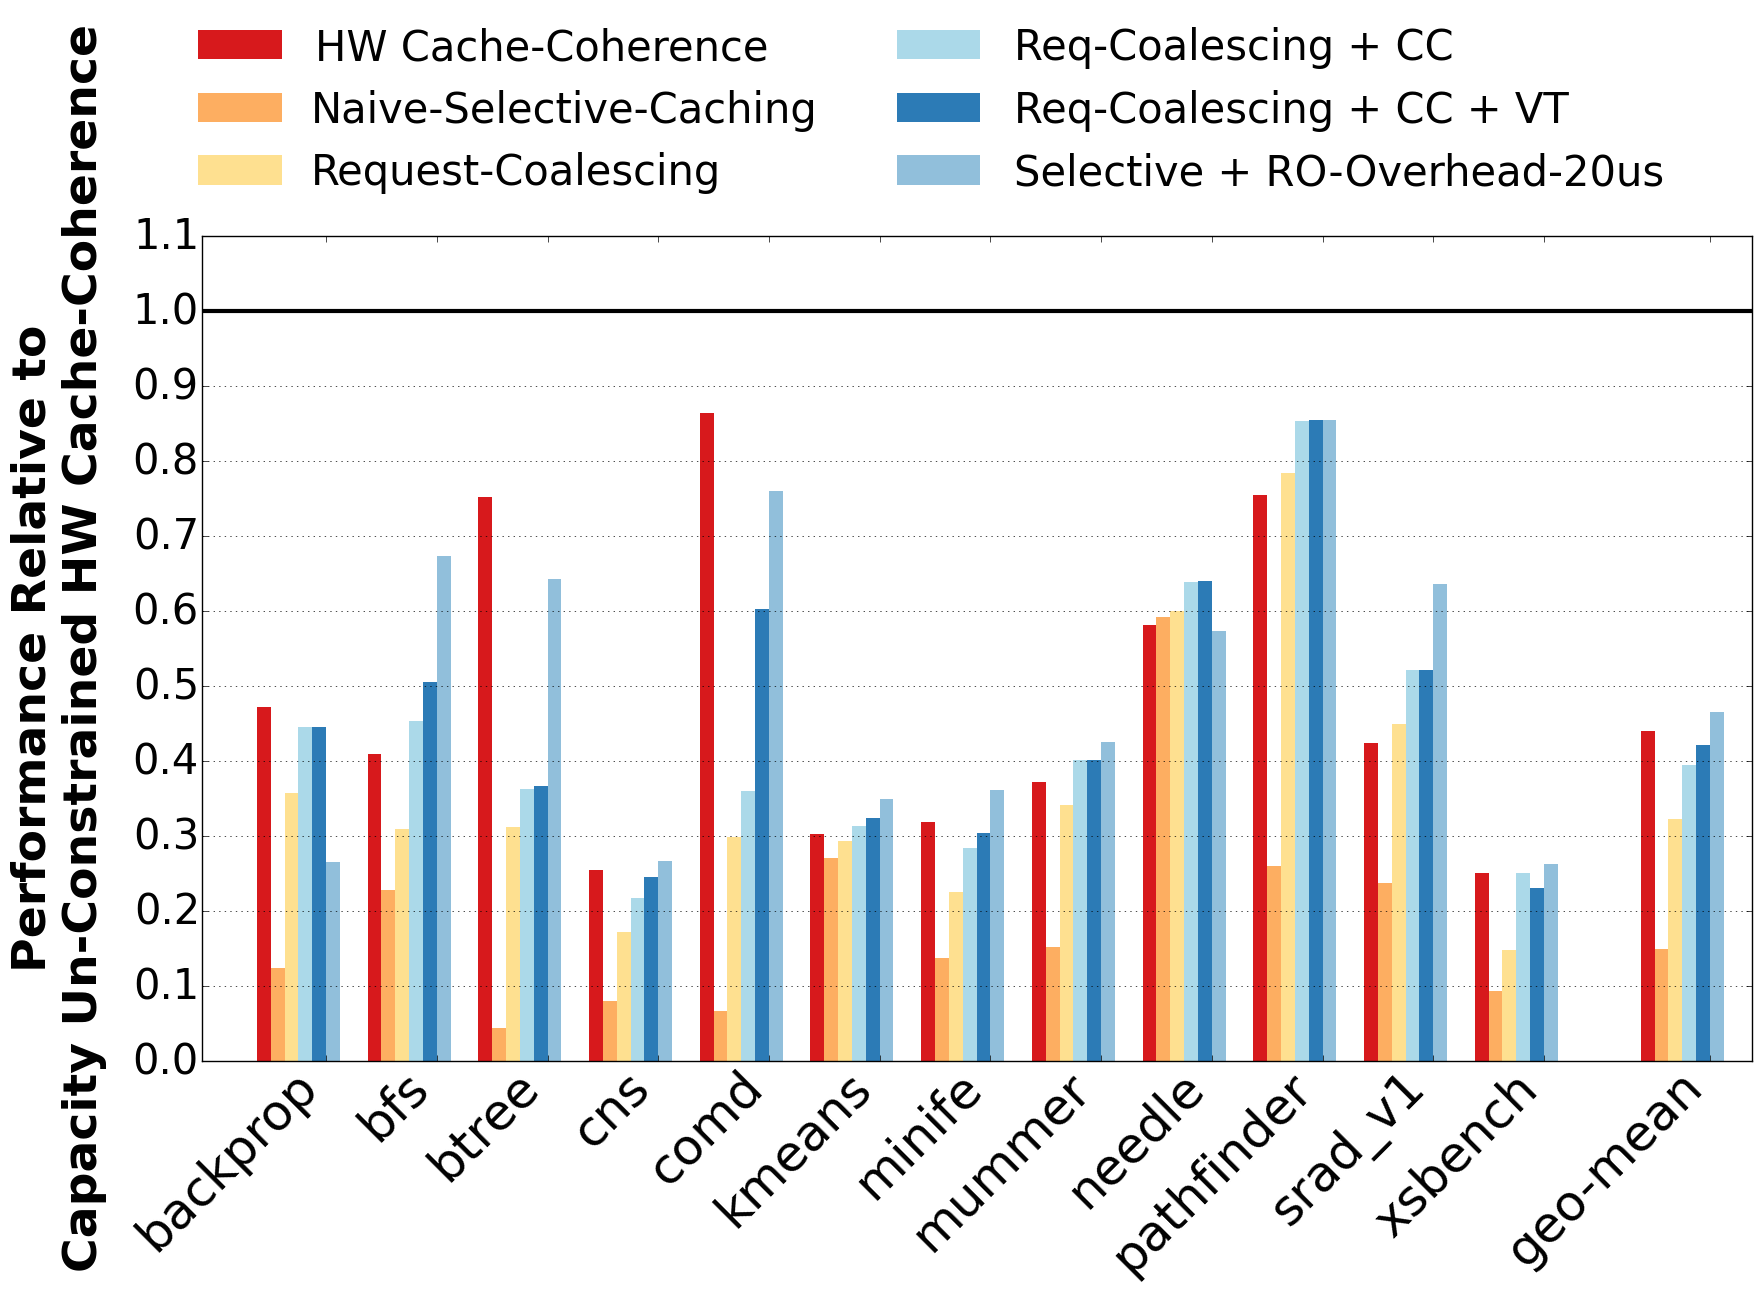
\includegraphics[width=1.0\columnwidth]{figures/capacityconstrained.png}
% % \caption{GPU performance under memory capacity constraints. (CC: Client-Cache,
% % VT: Variable-sized Transfer Units)}
% % \label{fig:capacityconstrained}
% % \end{figure}
% % 
% % In this work, we have primarily investigated a system where bandwidth-aware 
% page placement
% % provides an initial page placement that has been shown to have optimal 
% performance~\cite{Agarwal2015}.
% % Bandwidth-aware page placement is based on the premise that the GPU will place 
% pressure on
% % the CPU and GPU memory system in proportion to the number of pages placed in 
% each memory.  Proposals
% % like selective caching that change the on-chip caching policy of the GPU can 
% cause dramatic
% % shifts in the relative pressure placed on each memory system, effectively 
% changing the bandwidth-optimal 
% % placement ratio.  Although we do not evaluate this phenomenon in this work, 
% balancing
% % initial page placement with dynamic page migration to help compensate for the 
% lack of on-chip
% % caching is an area that needs further investigation.
% % 
% % \section{Related Work}
% % \label{related_work}
% % 
% % Cache coherence for CPUs has received great attention in the literature.
% % Recent proposals have started to explore intra-GPU and CPU--GPU cache 
% coherence.
% % 
% % \textbf{CPU Systems:} Scalable cache coherence has been studied extensively 
% for CPU-based
% %  multicore systems. Kelm et al. show that scaling up coherence to hundreds
% % or thousands of cores will be difficult without moving away from pure
% % hardware-based coherence~\cite{Kelm2009,Hill92}, due to high directory storage
% % overheads and coherence traffic~\cite{Lebeck95,Cheng06}.  
% % Whereas some groups have
% % evaluated software shared memory implementations~\cite{Falsafi94,Hill92}, 
% Martin
% % et al. argue that hardware cache coherence for mainstream processors is here 
% to
% % stay, because shifting away from it simply shifts the burden of correctness 
% into
% % software instead of hardware~\cite{Martin2012}. Nevertheless, disciplined 
% programming
% % models coupled with efficient hardware implementations are still being 
% pursued~\cite{choi2011,Sung2013,Sung2015}.
% % 
% % Self-invalidation protocols have been proposed to reduce invalidation traffic 
% and reduce
% % coherence miss latency~\cite{Lebeck95,Lai2000}. Our selective caching request 
% coalescing scheme uses a similar idea,
% % discarding a block immediately after fulfilling requests pending at the MSHR.
% % Other proposals have classified data into private, shared, and
% % instruction pages and have devised techniques to curtail coherence 
% transactions
% % for private data~\cite{Pugsley2010,Hardavellas2009,Cuesta2011,Ros2012}. We 
% instead classify
% % pages into read-only versus read-write and exploit the fact that read-only 
% data
% % can be safely cached in incoherent caches.
% % 
% % Ros and Kaxiras~\cite{Ros2012} have proposed a
% % directory\hyp{}less\slash{}broadcast\hyp{}less coherence protocol where all 
% shared
% % data is self\hyp{}invalidated at synchronization points. In this scheme,
% % at each synchronization point (e.g., lock acquire/release, memory barrier) all
% % caches need to be searched for shared lines and those lines have to be
% % flushed---an expensive operation to implement across hundreds of GPU caches 
% with data
% % shared across thousands of concurrent threads.
% % 
% % \textbf{Heterogeneous Systems and GPUs:} With the widespread adoption of GPUs 
% as a primary
% % computing platform, the integration of CPU and GPU systems has
% % resulted in multiple works assuming that CPUs and GPUs will eventually become
% % hardware cache-coherent with shared page
% % tables~\cite{power2014,Pichai2014,Agarwal2015,Agarwal2015b}.  CPU--GPU 
% coherence
% % mechanisms have been investigated, revisiting many ideas from distributed 
% shared
% % memory and coherence verification~\cite{Gelado2010,wu2014,Kaxiras2013}. Power 
% et
% % al.~\cite{Power2013} target a hardware cache-coherent CPU--GPU system by
% % exploiting the idea of region
% % coherence~\cite{Cantin2005,Alisafaee2012,Moshovos2005,Zebchuk2007}. They treat 
% the CPU and the
% % GPU as separate regions and mitigate the effects of coherence traffic by
% % replacing a standard directory with a region directory. 
% % In contrast, we identify that CPUs and GPUs need not be cache-coherent; 
% % the benefits of unified shared memory can also be achieved via selective 
% caching, which has lower
% % implementation complexity.
% % 
% % Mixing incoherent and coherent shared address spaces has been explored before 
% in the context of
% % CPU-only systems~\cite{Huh04} and the appropriate memory model for mixed
% % CPU--GPU systems is still up for
% % debate~\cite{Lim2012,Hechtman2014,Hower2014,Gaster2015}.  Hechtman et 
% al.~propose 
% % a consistency model for GPUs based on release consistency, which allows
% % coherence to be enforced only at release operations.  They propose a 
% % write-through no-write-allocate write-combining cache that tracks dirty data
% % at byte granularity.  Writes must be flushed (invalidating other cached 
% copies) only 
% % at release operations.  Under such a consistency model, our selective caching 
% scheme 
% % can be used to avoid the need to implement hardware support for these 
% invalidations between
% % the CPU and GPU.
% % 
% % Cache coherence for GPU-only systems has been studied by
% % Singh et al.~\cite{Singh2013}, where they propose a timestamp-based hardware 
% % cache-coherence protocol to self-invalidate cache lines. Their scheme targets 
% % single-chip systems and would require synchronized timers across multiple 
% % chips when implemented in multi-chip CPU--GPU environments.
% % Kumar et al.~\cite{Kumar2015} examine CPUs and fixed-function accelerator
% % coherence, balancing coherence and DMA transfers to prevent data ping-pong.
% % Suh et al.~\cite{Suh2004} propose integrating different coherence
% % protocols in separate domains (such as MESI in one domain and MEI in 
% another). 
% % However, this approach requires invasive changes to
% % the coherence protocols implemented in both domains and
% % requires significant implementation effort by both CPU and GPU vendors.
% % 
% % \textbf{Bloom Filters:} Bloom Filters~\cite{Bloom1970} and Cuckoo
% % Filters~\cite{Pagh2004,fan2014} have been used by several
% % architects~\cite{Strauss2006,Zebchuk2009,Hongzhou2011} in the past. Fusion
% % coherence~\cite{wu2014} uses a cuckoo directory to optimize for power and area 
% in
% % a CMP system. JETTY filters~\cite{Moshovos2001} have been proposed for 
% reducing
% % the energy spent on snoops in an SMP system. We use a cuckoo filter to 
% implement
% % the GPU remote directory.

\vspace{-0.1in}
\section{Related Work}
Multi-GPU programming is commonly used for scaling GPU performance via integration 
of multiple GPUs at the system 
level~\cite{pascal-tesla-wp,dgx,intersect360,titan_supercomputer} for a 
rapidly growing pool of 
applications~\cite{coral,cudnn,Lavin15b,SimonyanZ14a}. Similarly, 
multi-socket and multi-node CPU installations have been employed and studied 
in context of high performance computing and datacenter 
applications~\cite{Intel:Xeon,IBM:Power,IBM:z196,AMD:Opteron}.
Multi-GPU programming requires explicit design for multiple GPUs
using SW APIs such as Peer-2-Peer access~\cite{NVIDIAP2P} or a combination of
MPI and CUDA~\cite{NVIDIAMPI}. These extensions require
unique programming experience and significant SW effort while adapting a
traditional GPU application to a multi-GPU system. In this paper
we execute single GPU applications on a NUMA multi-GPU system as if it was a single
larger GPU via hardware innovations and extensions to the driver software stack;
providing programmer and OS transparent execution, similarly to approaches
proposed in the past~\cite{Cabezas2015,lee2013transparent,ben2015memory}.

Modern multi-socket CPU and GPU systems leverage advanced interconnect
technologies such as NVLink, QPI and
Infinity~\cite{dgx,INTELQPI,AMDINFINITYFABRIC}. These modern fabrics utilize
high speed serial signalling technologies over unidirectional lanes
collectively comprising full-duplex links. Link capacity is
statically allocated at design time and usually is symmetric in nature. Asymmetric
network on chips and NUMA interconnects have been previously investigated
and deployed~\cite{ziabari2015asymmetric, phillips2014m7}. In this
paper we propose to dynamically re-allocate available link bandwidth resources
by using same system wiring resources and on-chip I/O interfaces, while
implementing both receiver and transmitter driver circuitry on each lane. This
approach resembles previously proposed tristate bi-directional bus
technologies~\cite{tri-state} or former technologies such as the Intel front-side
bus~\cite{fsb}, albeit with just two bus clients. However our proposal leverages fast
singled ended signalling while allowing a dynamically controlled
asymmetric bandwidth allocation via on-the-fly reconfiguration of the
individual lane direction within a link.

Static and dynamic cache partitioning techniques were widely explored in the
context of CPU caches and QoS
~\cite{ics2007,Herdrich2016CacheQF,pact06,qureshi-micro,jaleel-pact} For
example, Rafique et.~al~\cite{pact06} proposed architectural support for shared
cache management with quota-based approach. Qureshi et.~al~\cite{qureshi-micro}
proposed to partition cache space between applications. Jaleel et.~al~\cite{jaleel-pact} 
improved on this by proposing adaptive insertion
policies. Recently, cache monitoring and allocation technologies were added to
Intel Xeon processors, targeted for QoS enforcement via dynamic repartitioning
of on-chip CPU cache resources~\cite{Herdrich2016CacheQF} between applications.  
Efficient cache partitioning in the GPU has been explored in context of L1 caches
~\cite{li-priority-based} to improve application throughput. While dynamic cache 
partitioning has been widely used for
QoS and L1 utilization, to the best of our knowledge it has never been used
to try to optimize performance when caches are backed by NUMA memory
systems.

\section{Conclusions}
\label{conclusions}
Two paragraphs of best paper awards goes here.

% Introducing globally visible shared memory in future CPU--GPU systems
% improves programmer productivity and significantly reduces the barrier
% to entry of using such systems for many applications. 
% Hardware cache coherence can provide such shared memory and
% extend the benefits of on-chip caching to all system memory.
% \ignore{Hardware cache coherence in future CPU/GPU systems would allow the integration
% of the separate CPU and GPU programming paradigms under a single
% uniform model, leveraging the benefits of on-chip caching for all
% memory within the system.}  However, extending hardware cache coherence 
% throughout the GPU places enormous
% scalability demands on the coherence implementation.  Moreover, integrating
% discrete processors, possibly designed by distinct vendors,
% into a single coherence protocol is a prohibitive engineering and
% verification challenge.  
% 
% We demonstrate that CPU--GPU hardware cache coherence is not needed to achieve the
% simultaneous goals of unified shared memory and high GPU performance.  
% We show that \textit{selective caching} with request coalescing,
% a CPU-side GPU client cache and variable-sized transfer units
% can perform within 93\% of a
% cache-coherent GPU for applications that do not perform fine
% grained CPU--GPU data sharing and synchronization. We also show that promiscuous
% read-only caching benefits memory latency-sensitive applications by using
% OS page-protection mechanisms rather than relying on hardware cache coherence.  Selective caching
% does not needlessly force hardware cache coherence into the GPU memory system,
% allowing decoupled designs that can maximize CPU and GPU performance, while
% still maintaining the CPU's traditional view of\ignore{ a hardware coherent} the
% memory system.

\bibliographystyle{IEEEtran}
\bibliography{main}
\end{document}
